\documentclass{article}

\usepackage[inner=3cm,outer=3cm]{geometry} %left=4cm,right=2cm would be equivalent
\usepackage[utf8]{inputenc}
%\usepackage{hyperref}
%\usepackage{natbib}
\usepackage{amsmath}
\usepackage{parskip}
\usepackage{graphicx}
\usepackage{placeins}
\usepackage{float}
\usepackage{listings}
\usepackage{color}

\definecolor{dkgreen}{rgb}{0,0.6,0}
\definecolor{gray}{rgb}{0.5,0.5,0.5}
\definecolor{mauve}{rgb}{0.58,0,0.82}


\lstset{frame=tb,
  language=Fortran,
  aboveskip=3mm,
  belowskip=3mm,
  showstringspaces=false,
  columns=flexible,
  basicstyle={\small\ttfamily},
  numbers=none,
  numberstyle=\tiny\color{gray},
  keywordstyle=\color{blue},
  commentstyle=\color{dkgreen},
  stringstyle=\color{mauve},
  breaklines=true,
  breakatwhitespace=true,
  tabsize=3
}

\lstdefinestyle{pstyle}{frame=tb,
  language=Python,
  aboveskip=3mm,
  belowskip=3mm,
  showstringspaces=false,
  columns=flexible,
  basicstyle={\small\ttfamily},
  numbers=none,
  numberstyle=\tiny\color{gray},
  keywordstyle=\color{blue},
  commentstyle=\color{dkgreen},
  stringstyle=\color{red},
  breaklines=true,
  breakatwhitespace=true,
  tabsize=3
}


\usepackage{xcolor}
\newcommand{\code}[1]{\texttt{#1}}
\title{SVE-R}
\author{octavia Crompton}
\date{November 2018}

\begin{document}
\tableofcontents		
%\maketitle

\section{Introduction}

The SVE-R model couples the 2D Saint Venant Equations (SVE), also known as the shallow water equations, to a 1D Richards equation solver for infiltration.  The SVE solver is adapted from the model presented in Bradford and Katopodes (1999), referenced here as BK1999, which uses a finite volume discretization to solve the 2D SVE on an arbitrary mesh consisting of quadrilaterals.   The SVE solver uses Hancock's predictor-corrector method  to achieve 2nd order accuracy in time, and Roe's Approximate Riemann Solver along with a MUSCL reconstruction of primitive variables to obtain 2nd order accuracy in space.   The model can handle a variably sloping bed, as well as wetting and drying in the domain.

The principal difference between  BK1999's model and the SVE-R model documented here is that infiltration is represented by solving Richards equation in 1D at each grid cell and timestep.  The 1D Richards equation was implemented using the algorithm described by  \textit{Celia et al.} (1990).  


The core of the model is implemented in Fortran  (\code{dryR.for}), and Python scripts are provided to write and read the Fortran files.
  
This document is divided into the following sections:

\begin{itemize}
	\item Section \ref{SVE} provides a brief summary of the Saint Venant Equations, Richards Equation and how the equations are coupled.
	\item Section \ref{SVE_solver} overviews the Fortran code, including the  au	xiliary input/output files and important subroutines.
	\item Section \ref{domain} describes the simulation domain (i.e. the specific scenario of rain driven overland flow on patchily vegetated hillslopes which the model is configured to solve).
	\item  Section \ref{python_wrap} overviews of the Python wrapper scripts,  which can be used to write the Fortran input files, compile and execute the Fortran code, and read and visualize the results.
	\item Section \ref{select_examples} lists the simulation examples provided as templates.
	\item Section \ref{emulator} briefly introduces the emulator feature code.
\end{itemize}		  

\textbf{DISCLAIMER}:
The model is published with the permission of Bradford and Katopodes, and the documentation closely follows BK1999 and  \textit{Bradford and Katopodes} (2001), henceforth BK2001. For further information and detail, please refer to these papers.  Parts of Sections \ref{SVE} and \ref{SVE_solver} are reproduced verbatim from BK1999 and BK2001, because their wording is are clearer and more precise than ours would be.  We are not claiming that the SVE solver is original work.  Also note that the original BK1999 model is not available open source.
  
\section{Background: equations and numerical methods }
\label{SVE}

\subsection{The 2D Saint Venant Equations (SVE)}
The SVE are written in integral form:

\begin{equation}
	\dfrac{\partial}{\partial t} \int_\Omega \mathbf{U} d\Omega + \oint_\partial (\mathbf{F} dy - \mathbf{G} dx ) = \int_\Omega \mathbf{Q} d\Omega
\end{equation}

where $\mathbf{U}^T = (h, hU, hV) $ is the vector of conservative variables. 


\[ \mathbf{F} = 
\begin{bmatrix}
	h U  \\
	h U^2 + \frac{1}{2} g h^2 \\
	h U V \\
\end{bmatrix}  ; \quad
\mathbf{G} = 
\begin{bmatrix}
	h V \\
	h U V \\
	h V^2 + \frac{1}{2} g h^2 \\	
\end{bmatrix}  
\]

where $h$ is the flow depth,  $z$ is the bed elevation, $U$ and $V$ are the vertically averaged velocities in the $x$ and $y$ directions, respectively. 
The source terms are defined as:


 \[ \mathbf{Q} = 
 \begin{bmatrix}
	p - i  \\[.1cm]
	- g h \dfrac{\partial z}{\partial x} - g h  S_{f,x} + \dfrac{u(p-i)}{2}\\[.15cm]
	- g h \dfrac{\partial z}{\partial y} - g h  S_{f,y} + \dfrac{v(p-i)}{2}\\[.15cm]
\end{bmatrix} 
\]

where $p$ is the rainfall rate,   $i$ is the infiltration rate of water into the bed, and $S_{f,x}$ and $S_{f,y}$ are the $x$ and $y$ components of the friction slope. 


\subsection{SVE numerical methods}

 The model is adapted from  \textit{Bradford and Katopodes} (1999), referred to here as BK1999,  which uses predictor-corrector time-stepping to provide a second-order accurate solution.
%  The following summary of the numerical methods is adapted from \textit{Bradford and Katopodes} (1999), where a better and more complete explanation can be found. 
  
  A predictor solution is computed at  time level $n + 1/2$ by solving the primitive equations in generalized coordinates, and a corrector is computed at the $n + 1$ time level by solving the integral equations.  
   
 \subsubsection*{Predictor Step}

In generalized coordinates, the SVE  are given as: 

\begin{equation}
\dfrac{\partial \mathbf{W}}{\partial t} + 
	\mathbf{A}_W	\dfrac{\partial \mathbf{W}}{\partial \xi} + 
	\mathbf{B}_W	\dfrac{\partial \mathbf{W}}{\partial \eta} =
	\mathbf{Q}_W
\label{predictor}
\end{equation}

\noindent where $\xi$ and $\eta$ are in the directions of increasing $j$ and $k$ indices, respectively.
The  $j$, $k$ indices indicate the column and row numbers of a given cell, respectively (see Figure \ref{coords} schematic).
$\mathbf{W_T} = [h, U, V]$ is the array of primitive variables, and the matrices $\mathbf{A}_W$ and $\mathbf{B}_W$ are defined as:

\[ \mathbf{A}_w = 
\begin{bmatrix}
    U_{\xi} & h \xi_x & h \xi_{y} \\
    g \xi_x &    U_{\xi}  & 0    \\
    g \xi_y &   0   & U_{\xi}    \\    
\end{bmatrix} \quad \mathbf{B}_w = 
\begin{bmatrix}
    U_{\eta} & h \eta_x    & h \eta_{y} \\
    g \eta_x &    U_{\eta}  & 0    \\
    g \eta_y &      0       & U_{\eta}    \\    
\end{bmatrix} 		
\]	


\noindent where $U_{\xi} = U \xi_x  + V \xi_y $ and $U_{\eta} = U \eta_x  + V \eta_y $.
$\xi_x$,  $\xi_y$,  $\eta_x$ and  $\eta_y$ are the grid transformation metrics for mapping $x$ and $y$ to $\xi$ and  $\eta$. In Cartesian coordinates, the generalized coordinates simplify to: $\xi  = x$ and  $\eta  = y$.

The predictor solution in cell $j$, $k$ at $t + \Delta t/2$  is given as:

 
\begin{equation}
\mathbf{W}_{j,k}^{n+1/2} = \mathbf{W}_{j,k}^{n}
- \frac{\Delta t}{2} (
	\mathbf{A}_W \overline{\Delta \mathbf{W}}_\xi+
	\mathbf{B}_W \overline{\Delta \mathbf{W}}_\eta-
	\mathbf{Q}_W)_{j,k}^{n+1/2}
\label{predictor}
\end{equation}


\noindent where the overbar denotes a cell-average gradient of $\mathbf{W}$ in cell $j$, $k$,  which is computed with a flux limiter (nonlinear average) in order to preserve solution monotonicity.  Flux limiters  become first-order accurate near discontinuities while remaining second-order accurate elsewhere, and several options are included in the code, described in Section \ref{SVE_solver}.

 \begin{figure}[h]
 \centering
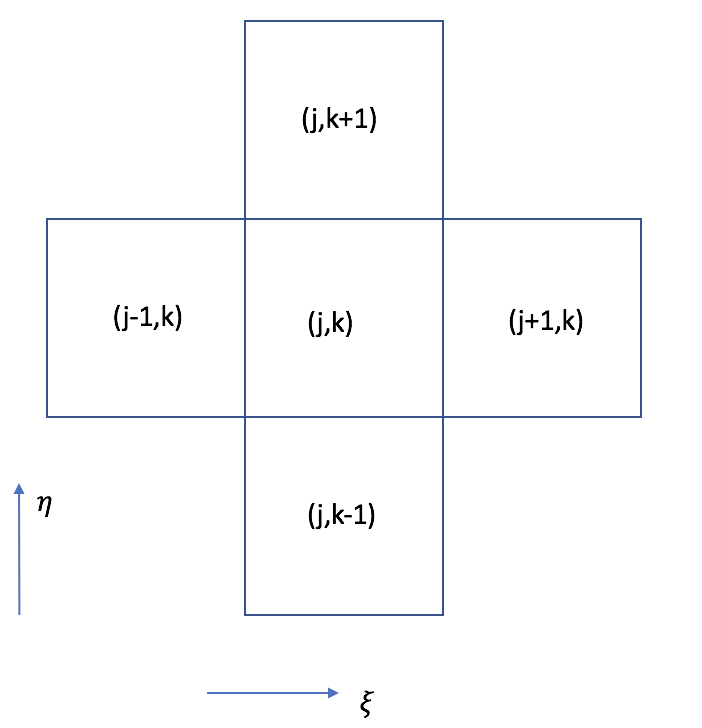
\includegraphics[width=15pc]{grid/coords.png}
 \caption{Sketch of a computational cell, after BK Figure 2.}
 \label{coords}
 \end{figure}
  

 \subsubsection*{Corrector Step}
 
 The corrector solution is obtained from the conservative form of the governing equations.
 
 The predictor solutions are reconstructed to the left and right of each cell face using the monotone upstream scheme for conservation laws (MUSCL), which achieves second-order spatial accuracy.  The reconstructed predictor values define a Reimann problem at each cell face, which are used to compute the interfacial fluxes:
 
\begin{equation} 
	\dfrac{\mathbf{U}_{j,k}^{n+1} -\mathbf{U}_{j,k}^{n}}{\Delta t} 
	+ \dfrac{1}{\Omega_{j,k}} \big[ 
		- \mathbf{F}_{\perp 1}^{n+1/2} \Delta s_1
		+ \mathbf{F}_{\perp 2}^{n+1/2} \Delta s_2
		+ \mathbf{F}_{\perp 3}^{n+1/2} \Delta s_3
		- \mathbf{F}_{\perp 4}^{n+1/2} \Delta s_4		
	\big] = \mathbf{Q}^{n+1/2}
\end{equation}

\noindent where $\mathbf{Q}$ and $\mathbf{U}$ are the cell-center values in cell $j,k$ with area $\Omega$, $\mathbf{F}$ and $\mathbf{G}$ are the average boundary values on each cell face, and $\delta s$ is the length of the cell faces.
The indices 1 through 4 denote the four cell faces: index 1 corresponds to the bottom cell face, and the remaining cell faces are numbered in counter-clockwise order.

The flux $\mathbf{F}_\perp$  is normal to the cell boundary and positive in the direction of increasing cell coordinates.  $\mathbf{F}_\perp$  is defined as:

\[ \mathbf{F}_\perp = 
\begin{bmatrix} 
    h u_\perp \\[0.1cm]
    h u u_\perp + \frac{1}{2} g h^2 \cos \phi   \\[0.1cm]
    h v u_\perp + \frac{1}{2} g h^2 \sin \phi   \\[0.1cm]    
\end{bmatrix}  		
\]	

where $u_\perp$ is the velocity perpendicular to the cell face, and $\phi$ is the angle between the face normal vector and the $x$-axis.

The fluxes are evaluated using a Godunov-type upwind scheme in which a Riemann problem is solved across each cell face, using the method of Roe (1981).  Further details can be found in BK.


\subsubsection*{The source term }

The source term $\mathbf{Q}$ contains the parameterization of the surface roughness (via the friction slope $S_f$  and the lateral inputs (rainfall $p$ and infiltration $i$).  Infiltration is independently modeled at each timestep and grid cell with the 1D Richards equation, described in the next subsection.
  
 The friction slope is specified in the generalized form: 

\begin{eqnarray} \nonumber
S_{f,x} = \bigg( \dfrac{\alpha  U}{h^m}\bigg)^{1/\eta} \dfrac{|U|}{U}; \quad
S_{f,y} = \bigg( \dfrac{\alpha  V}{h^m}\bigg)^{1/\eta} \dfrac{|U|}{V}
\end{eqnarray}

\noindent where $\alpha$ is a  roughness parameter, and $m$ specifies the flow regime ($m=2$ for laminar flow, 1/2 for turbulent flow).   $\eta$=1/2 for most roughness schemes, with the exception of laminar flow, for which $\eta$=1.  For Manning's equation, $\alpha = n$, $m=2/3$ and $\eta=1/2$:

\begin{eqnarray} \nonumber
S_{f,x} =  \dfrac{n^2 U}{h^{4/3}} |U|; \quad
S_{f,y} = \dfrac{n^2 V}{h^{4/3}} |U|
\end{eqnarray}

\noindent More generally, with $\eta=1/2$:
\begin{eqnarray} \nonumber
S_{f,x} = \dfrac{\alpha^2 }{h^m}  U |U|; \quad
S_{f,y} = \dfrac{\alpha^2 }{h^m} V |U|
\end{eqnarray}


\subsection{Richards equation}

Richards equation is solved following the approach outlined by Celia et al. (1990), which involves a backward Euler approximation in time coupled with a simple Picard iteration scheme.  
The solver used the discrete approximation of the  mixed $H$-$\theta$ form: 

\begin{equation} 
	\dfrac{\partial \theta}{\partial t} - \nabla \cdot K \nabla H - \dfrac{\partial K}{\partial z} = 0
\label{richards}
\end{equation}

\noindent where $z$ denotes the vertical dimension (assumed positive upwards),  $\theta$ is the soil moisture content, $H$ is the matric potential and $K$ is the unsaturated hydraulic conductivity.
 $\theta$ and $H$ are related via the Van Genuchten water retention curve. The volumetric soil moisture content, $\theta$, and effective saturation, $S_e$, are computed as:

\begin{eqnarray} \nonumber
\theta = \dfrac{\theta_S – \theta_R}{1 + (\alpha|H|)^n)^m} + \theta_R
\label{vanG_eqn}
\end{eqnarray}

\begin{eqnarray} \nonumber
S_e = \dfrac{\theta – \theta_R}{\theta_S – \theta_R}
\label{Se}
\end{eqnarray}

 where $\theta_S$ and  $\theta_R$ are the saturated and residual soil moisture content; $n$ is a measure of the pore size distribution; $m=(1-1/n)$; and $\alpha$  is related to the inverse of the air entry suction.  The unsaturated hydraulic conductivity $K(\theta)$ is computed as:

\begin{eqnarray}
K = K_s \sqrt{S_e} [1 – (1 – S_e^{1/m})^m]^2
\label{K}
\end{eqnarray}

where $K_s$ is the saturated hydraulic conductivity.
The infiltration rate is solved with Darcy's law:

\begin{equation}
q =-  K \bigg(\dfrac{\partial H}{\partial z} + 1\bigg)
\label{darcy}
\end{equation}

where the 1  (second term) on the RHS reflects the fact that $H$ is the matric head, as opposed to the hydraulic head.

\subsection{Coupling the SVE and Richards equation models}

The model components are coupled at each grid cell in two steps: the depth from the SVE solver provides the surface boundary condition to the Richards equation solver, and the infiltration rate from the Richards equation solver is used by the SVE source term. This requires that several cases be accounted for: (1) no rain and no ponding, (2) rain but no ponding, and (3)  ponding (with or without rain).   In case (1), a no flux boundary condition is applied at the surface.
 In case (2), the Richards equation solver computes a potential infiltration rate ($PI$), defined as the infiltration rate that would occur with $H=0
 $ cm at the surface, and compares this value to the rainfall intensity, $p$.  If $p$ exceeds the potential infiltration rate, ponding begins and the  boundary condition switches to case (3).  Otherwise, the potential infiltration rate is greater than $p$, and $i=p$. Finally, in case (3), the upper boundary condition $H$ is equal to the ponding depth $h$.  These cases are schematically illustrated in Figure \ref{richardgrid}.
 
 	
 \begin{figure}[h]
 \centering
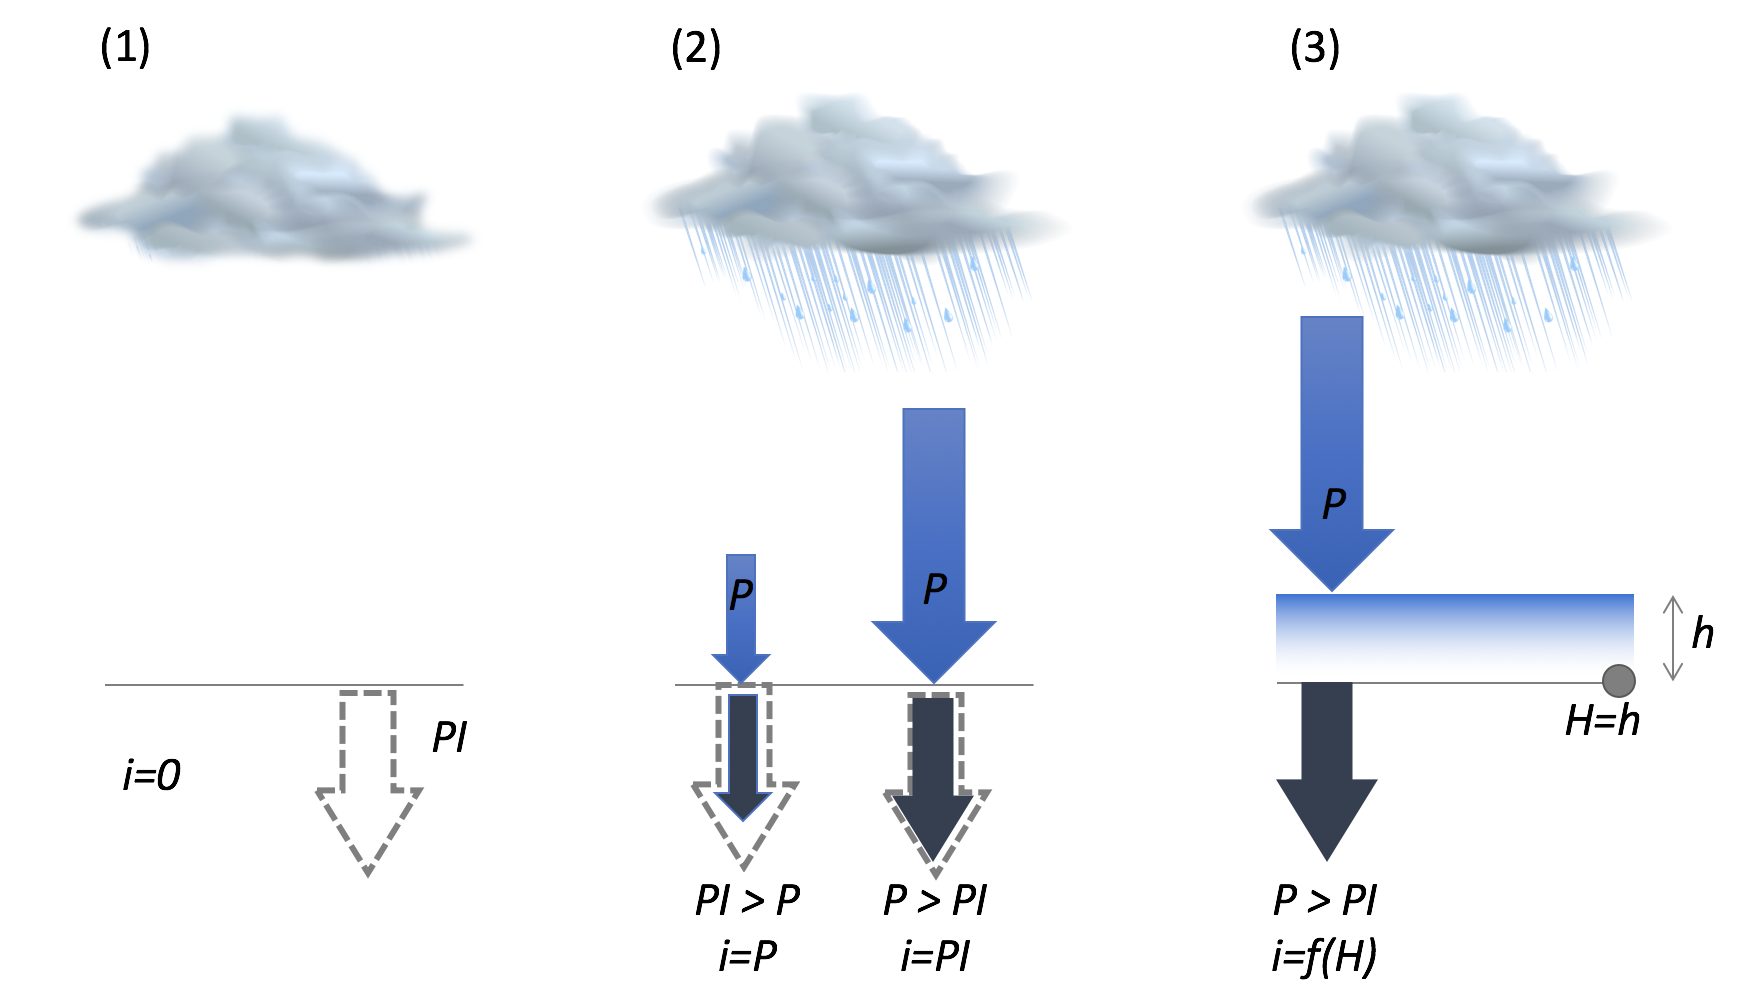
\includegraphics[width=20pc]{grid/richards.png}
 \caption{Schematic to illustrate the boundary condition cases for Richards equation. $PI$ is the potential infiltration rate, which is computed to determine whether the rain intensity exceeds the infiltration capacity of the soil (in which case ponding occurs).}
 \label{richardgrid}
 \end{figure}	


\newpage

\section{SVE-R Fortran code}

This section outlines the structure of the Fortran code, how to compile and execute it, and the required input files.  Further details on the the SVE and Richards equation solvers, particularly those relating the mathematical equations in Section 2 to the Fortran code, can be found in Appendix A.

\label{SVE_solver}


\subsection{SVE-R model structure}

\code{dry.f} can be compiled and executed from an Mac s terminal with:

\hspace*{8mm} \code{gFortran -o ./sw  -framework accelerate ./dry.for} \\
\hspace*{8mm} \code{.sw} \\

 where \code{.sw} is the name of the executable.  \code{dry.f} interacts with a number of auxiliary files (see screenshot in Figure \ref{files}), including:

\begin{itemize}
	\item \code{\code{dry.inc}}: specifies common variables used by \code{dry.f}  (a number of variables are ``common" variables, and not explicitly returned by the Fortran subroutines). 
	\item \code{input}:  contains files to initialize \code{dry.f}.
	\item \code{output}: contains output files created by \code{dry.f}.
	\item \code{params.json}: user-supplied parameter dictionary.
	\item \code{.sw}: the compiled Fortran executable.
	\item \code{.ipynb} files: Jupyter notebooks to visualize the simulation outputs.
\end{itemize}
 


 \begin{figure}[h]
 \centering
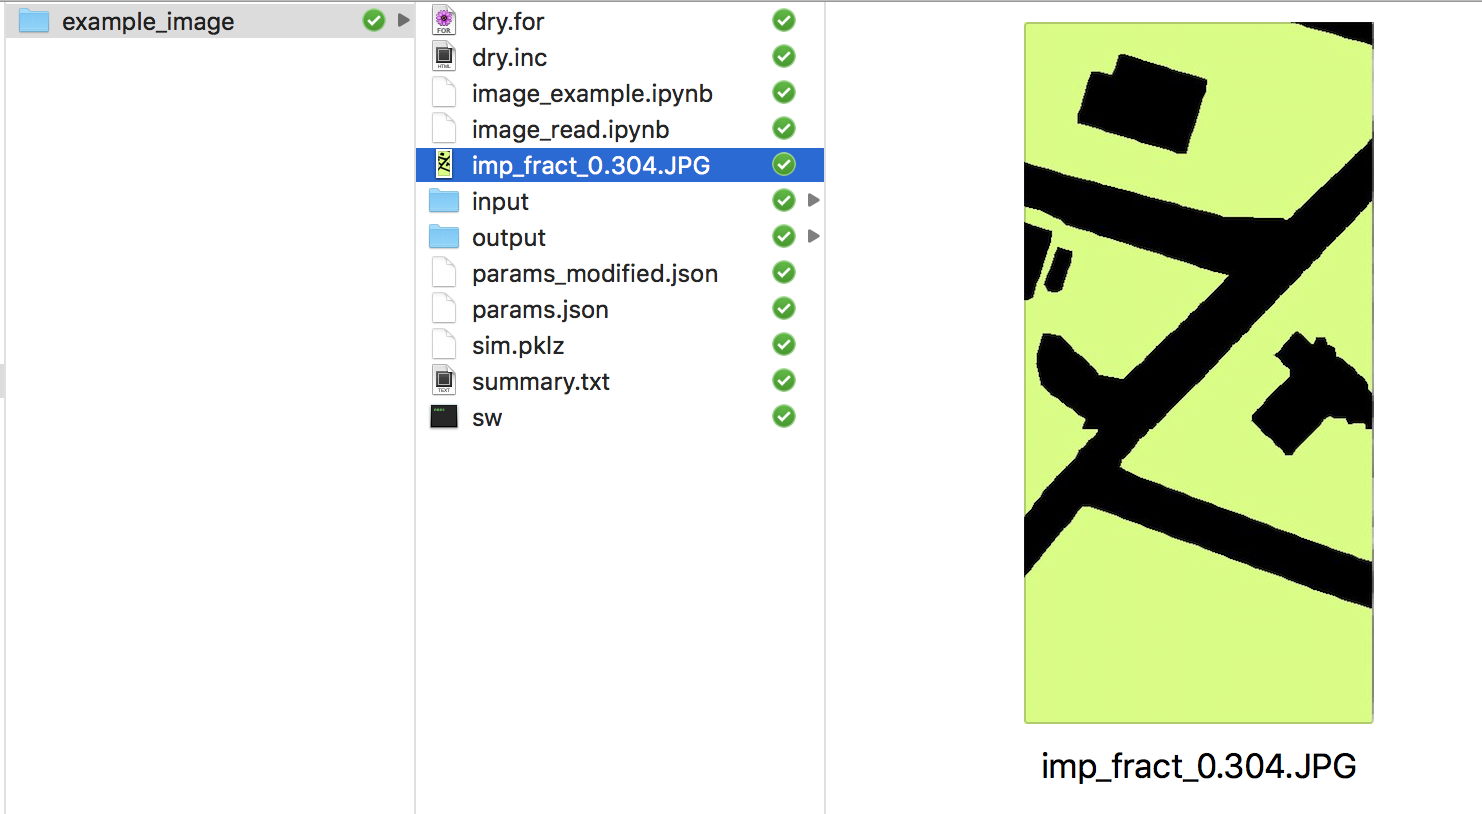
\includegraphics[width=25pc]{grid/files.png}
 \caption{Auxiliary files associated with \code{dry.f}.}
 \label{files}
 \end{figure}


Figure \ref{summary} summarizes the organization of \code{dry.f}, which can be divided into main two steps: (1) initializing and (2) executing a time loop.   The following subsections describe the model components in greater detail.


\begin{figure}[h]
 \centering
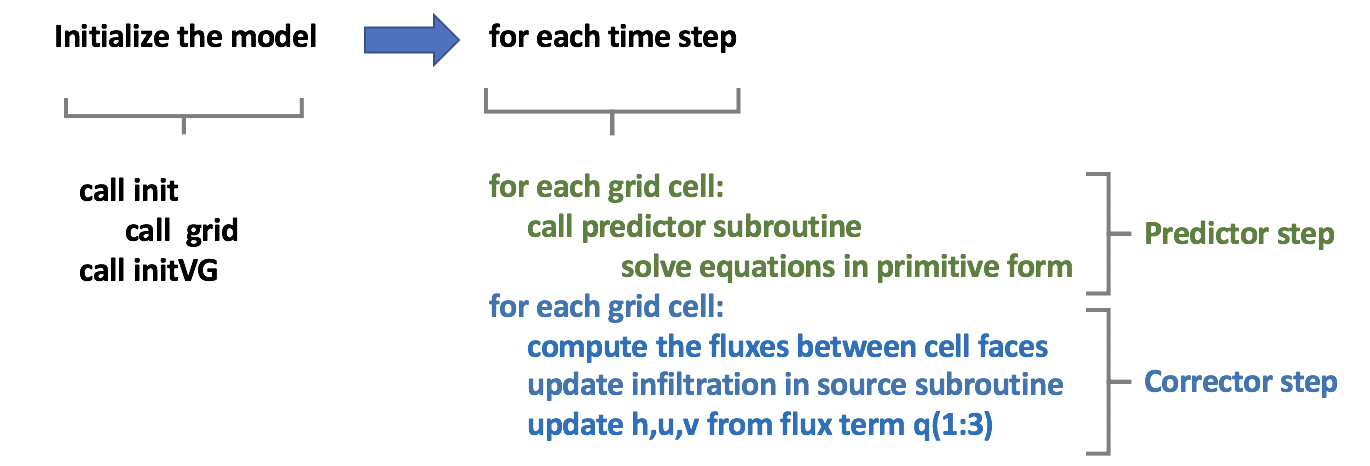
\includegraphics[width=30pc]{grid/summary.png}
 \caption{Summary of the SVE-R model structure in \code{dry.f}.}
 \label{summary}
 \end{figure}


\subsection{Model set-up}
\label{SVEinit}
	
The \code{init} subroutine initializes the SVE component of the model,  which involves reading a number of scalar parameters from  \code{params.dat} and setting up the simulation grid.
 The infiltration parameters are initialized by the subroutine \code{initVG}.  The following briefly describes the input files, and further details are included in Appendix B (including an  example of a  2$\times$2 grid).
  
\subsubsection*{Input files}

The required input files are:

\begin{itemize}

	\item \code{params.dat}:  specifies a number of scalar parameters (read by the \code{init} subroutine).  

	\item \code{coords.dat}: contains the $x$,$y$,$z$ coordinates at the cell nodes.

	\item \code{boundary.dat}: describes the boundary types and locations.

	\item \code{veg.dat}: contains the vegetation pattern.

	\item \code{nodes.dat}: contains a list of the node numbers surrounding each grid cell.

	\item \code{vanG.dat}: Van Genuchten parameters and initial $H$ as a function of depth for vegetated and bare soil cells. 

\end{itemize}

See Appendix B for further details and examples.



\subsubsection*{Grid variables}

\begin{itemize}
	\item \code{nn}: space allocated to the grid (\code{nn>np}).
	\item  \code{np}:  the number of cell nodes. 
	\item \code{x(nn), y(nn), zz(nn)}: $x,y,z$ coordinates of the cell nodes.  \\[0.1cm]
		\code{x,y,zz} are read as 1D arrays, and interpolated to a 2D grid with the help of the nodes file \code{nodes.dat}.
		\item  \code{xc, yc, zc}: coordinates at the cell centers, with dimensions \code{(ncol, nrow)}

	\item \code{nop(nx,ny,4)}: node numbers defining each grid cell (see Figure \ref{nodes}).  

	\item \code{inum}: number of boundary interfaces of each cell.
	\item \code{itype}:  interface type of each cell boundary (1 for wall boundaries, 0 for open boundaries...).  
	\item \code{ipos}: position of each cell boundary (1 for lower boundaries, 2 for right boundaries...).
\end{itemize}


 \begin{figure}[h]
 \centering
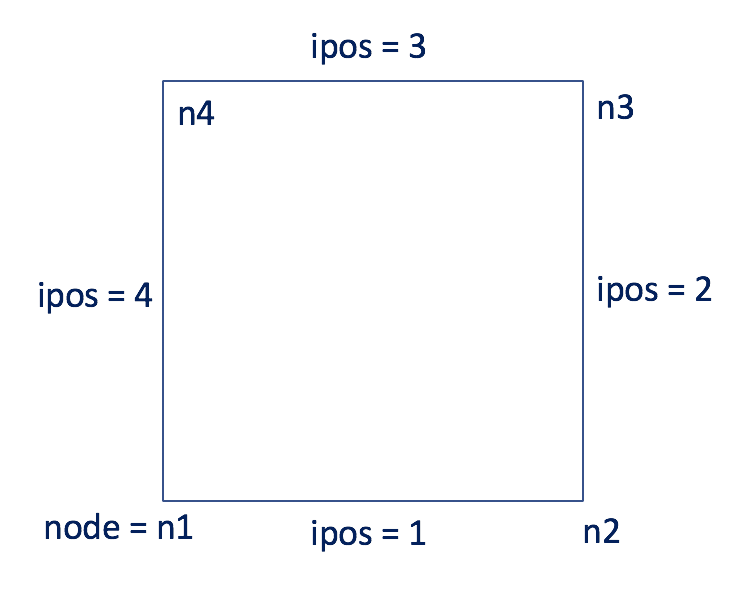
\includegraphics[width=15pc]{grid/boundaries.png}
 \caption{Schematic of the nodes and boundary naming convention. }
 \label{nodes}
 \end{figure}
 



\subsection{Model output}

 \code{dry.f} saves the following  files in the \code{output} subfolder.
Most variables are saved at intervals of  \code{dt\_p}, to limit the size of the output files, with the exception of the hydrograph, which is saved at 1 second resolution.   
\begin{itemize}
	\item \code{dvol.out}:  output file to check mass balance. Read by function \code{get\_dvol} in \code{output\_dry.py}.
	\item \code{fluxes1234.out}: lateral boundary fluxes, grouped by boundary  position (i.e. boundary positions 1-4).  
	\item \code{h.out}: primitive variables $h$, $U$, and $V$, infiltration $I$ and interfacial fluxes (saved at every grid-cell)
	\item \code{summary.out}: summarizes ponding time, runtime, final time, and if applicable, the reason for an early exit (i.e. no more water, AMAX too big) 
	\item \code{hydro.out}: hydrograph at 1 second time resolution (m$^3$/s).  
	\item \code{ptsTheta.out}: soil moisture profiles at two points, one vegetated and one bare. 
	\item \code{time.out}: file containing the max CFL number at each timestep.
\end{itemize}

\subsection{Principal model components (\code{dry.f} subroutines)}

This section provides a high level summary of the main model components (i.e. \code{dry.f} subroutines) and how they connect.  Further information and details can be found in Appendix A.

\subsubsection*{The predictor step}

The \code{predict} subroutine is called at each cell to compute \code{hp}, \code{up},  \code{vp},corresponding to $h^{n+1/2}$,$u^{n+1/2}$,$v^{n+1/2}$.   It modifies the common variables  \code{hp}, \code{up},  \code{vp}, \code{dh}, \code{du}, \code{dv}, \code{qs}.

\subsubsection*{Corrector step}

To compute the fluxes between the cell interfaces, the corrector step  calls the \code{fluxes} subroutine for each cell and for each interface. 

The interfacial cell fluxes at a given time-step are stored in the common variable \code{f(0:nx,0:ny,1:3,1:2)}, where the first two indices of \code{f} contain the $j,k$ coordinates, the third index correspond to the components of  $\mathbf{F_\perp}$, and the final index denotes the cell face (1 for vertical cell faces and 2 for horizontal).   
For example, \code{f(j,k,1:3,1)} represents the flux from cell $(j-1, k)$ to $(j, k)$, and
\code{f(j,k,1:3,2)} represents the flux from cell $(j, k-1)$ to $(j, k)$ (see Figure \ref{fluxes_specific}).
Calling \code{fluxes(j-1,j,k,k,1)} modifies \code{f(j,k,1:3,1)}  and calling \code{fluxes(j,j,k-1,k,2)} modifies \code{f(j,k,1:3,2)}.

 \begin{figure}[h]
 \centering
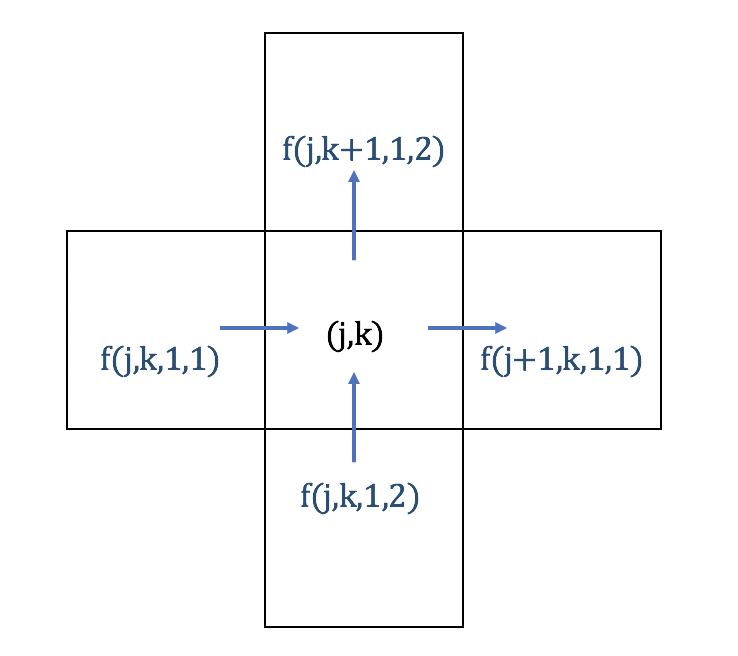
\includegraphics[width=15pc]{grid/fluxes_specific.png}
 \caption{Definitional sketch for the interfacial fluxes, indicating how the fluxes into and out of cell \code{(j,k)} are stored in the array \code{f(0:nx,0:ny,1:3,1:2)}}.
 \label{fluxes_specific}
 \end{figure}

\subsubsection*{Fluxes subroutine}

Within the \code{fluxes} subroutine, \code{fluxes(jl,jr,kl,kr,i1)} computes the flux from cell \code{(jl,kl)} to \code{(jr,kr)}, modifying the common variable \code{f(jr,kr,1:3,i1)}. 
\code{i1 = 1} indicates that the flux is between vertical cell faces, i.e. from cell \code{(j-1,k)} to \code{(j,k)}.
Similarly, \code{i1 = 2} indicates that the flux is between horizontal cell faces, i.e. from cell \code{(j,k-1)} to \code{(j,k)}.

 
\code{fluxes}  first reconstructs the predicted values to the left and right of each face (\code{hl,hr,ul, ur,vl,vr)} using the monotone upstream scheme for conservation laws (MUSCL).  These reconstructed predictor values define a Riemann problem at each cell face, and \code{fluxes} calls the \code{solver} subroutine to compute $\mathbf{F_{\perp I}}$ from BK1999 Equation 27, reproduced below:

\begin{equation*}
\mathbf{F_{\perp I}} =
	 \frac{1}{2} (\mathbf{F_{\perp L}} + \mathbf{F_{\perp R}} - \mathbf{\hat{R} |\hat{\Lambda}| \Delta \hat V  })
\end{equation*}


\subsubsection*{The \code{source} subroutine}

 The source term is computed with the subroutine \code{source}, which modifies the common variable \code{qs}.
  \code{source} is called in both the predictor and corrector steps; however, Richards equation is only solved in corrector step. 
 The input arguments are the  cell indices \code{j,k}, the primitive variables, and an indicator variable \code{lstep} for the step type (\code{lstep = 0} for the predictor step and 1 for the corrector step.		
 
In the predictor step, \code{source} is called for each cell before updating the predictor values (\code{hp,up,vp}).  \code{source} is similarly  called in the corrector step before updating the fluxes.

\subsubsection*{Infiltration details (corrector-step)}

In the corrector step, \code{source} calls the infiltration subroutines (\code{timestep} and \code{potential} to update the infiltration rate $i$ and the surface boundary conditions at cell \code{(j,k)}. 

\code{timestep} solves Richards equation at cell \code{(j,k)} and returns the updated $H$, $\theta$ and $K$, which \code{source} uses to compute the infiltration rate $i$. \code{potential} is used to prescribe the boundary conditions. 

Richards equation  is solved separately for each grid cell, and the 3-dimensional $H$, $\theta$ and $K$  fields are saved as the common variables \code{r8H} (cm), \code{r8Theta}, and  \code{r8K} (cm/s), respectively, with dimensions (\code{nrow} $\times$ \code{ncol} $\times$ \code{nz}).\\ 

The \code{potential} subroutine computes the infiltration that would occur with $H=0$ at the surface (\code{PI}), and is required for Richards case (2) in Figure \ref{richards}. Ponding does not occur until the \code{potential} subroutine determines that the rainfall exceeds to potential infiltration rate ($p>PI$). 	 When there is rain but no ponding (\code{depth=0} and \code{rain > 0}), the  \code{potential} subroutine is called to estimate a potential infiltration rate $PI$, defined as the infiltration that would occur with $H=0$ at the surface (in cm/s).   If the potential infiltration rate is less than the rainfall rate (\code{(PI .lt. rain*100)}), water accumulates on the surface.  In this case, the Richards boundary condition is switched to fixed $H$.	

\noindent From Darcy's law, the infiltration rate $i$ (cm/s) is computed as:
$$ i =  K \bigg(\frac{\partial H}{\partial z} + 1\bigg ) $$
which corresponds to \code{r8kt*((hdum(nz)-hdum(nz-1))/dz+1)} in \code{source}.


		




	
\section{The simulated domain}
\label{domain}
To simulate runoff/runon environments on patchily-vegetated hillslopes, several aspects of the BK model have been modified (in addition to coupling to a 1D Richards solver).  This section describes the simulated domain, as illustrated in Figure \ref{domain_schematic}.

 \begin{figure}[h]
 \centering
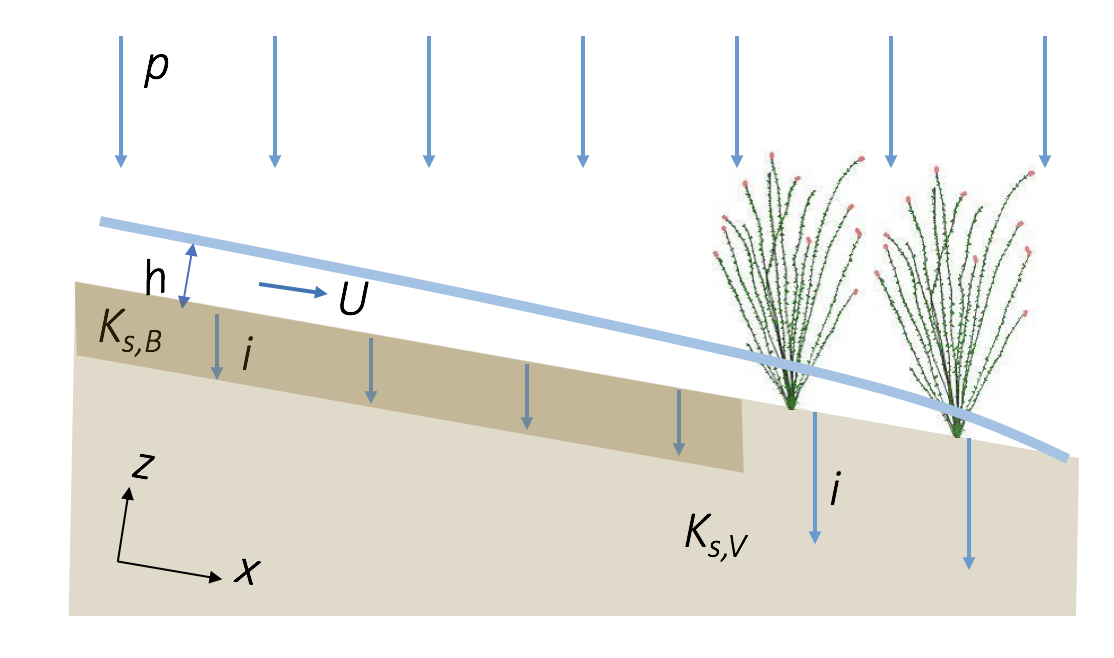
\includegraphics[width=20pc]{grid/domain_schematic.png}
 \caption{Schematic of the model domain.  The darker shading under the non-vegetated regions represents the surface crust.  $K_{s,V}$ and $K_{s,B}$  represent the saturated hydraulic conductivities of undisturbed soil and surface crust, respectively.}
 \label{domain_schematic}
 \end{figure}
 
 
First,  roughness parameters are specified separately for vegetated and bare cells. 
 The parameters for the resistance formula for vegetated cells are specified as  \code{alpha}, \code{eta} and \code{m}  ($\alpha$, $\eta$ and $m$), and for bare soil cells as  \code{alpha\_B}, \code{eta\_B} and \code{m\_B}  ($\alpha_B$, $\eta_B$ and $m_B$).
  The default soil parameters are Manning's equation with \code{alpha = 0.1}, and \code{alpha\_B = 0.03}.


The model is set up to specify rain-driven overland flow on a planar hillslope, for which the lateral boundaries are closed with the exception of the open boundary at the bottom of the hillslope.  An additional example  is provided for a fixed flux (subcritical) upslope boundary condition,  where the inflow boundary dimensions are equal to the entire upslope area.  Code for other boundary conditions is not provided, but can be implemented with modification to \code{input\_coords.py} (or directly to the Fortran input files).
For a fixed-flux upslope boundary, the `rain duration` \code{tr} also specifies that the time as which the inflow stops (i.e. the boundary changes from fixed flux to a wall boundary).  In the case of rain AND upslope inflow, for example, to simulate rain on a longer hillslope domain, the rain and inflow will end at the same time. 

The bare soil areas are represented by a two-layer model, where the upper, less-permeable  layer represents a surface crust.  With the exception of $K_{s}$, the van Genuchten parameters are the same between vegetated and bare cells. In the bare soil areas, $K_{s}$ of the lower soil layer is  equal to that in the vegetated patches (see Figure \ref{domain_schematic}).
The van Genuchten parameters and vertical structure of the soil can be modified in \code{input\_phi.py}.


\section{Python wrapper scripts}
\label{python_wrap}

\begin{itemize}
\item \code{write\_nodes(path, ncol, nrow)  }: writes the cell node indices to \code{input/nodes.dat}.  
    This function assumes that the grid is rectangular, and would need to be modified for a non-rectangular grid. 
       It saves \code{nop.dat}, which contains the indices of the nodes surrounding each cell face.
\item \code{build\_coords(params)}: constructs the \code{x,y,z} coordinates fields. 
\end{itemize}

%\noindent Note: \code{coords.pklz} stores the cell center coordinates in a Python readable file, and is not a Fortran input file.


Example Python scripts are provided to generate the Fortran input files, execute \code{dry.f} and read the outputs.   \code{call\_dry.py} is a control script which executes each of these components, as illustrated in the Figure \ref{schematic} schematic.

 \begin{figure}[h]
 \centering
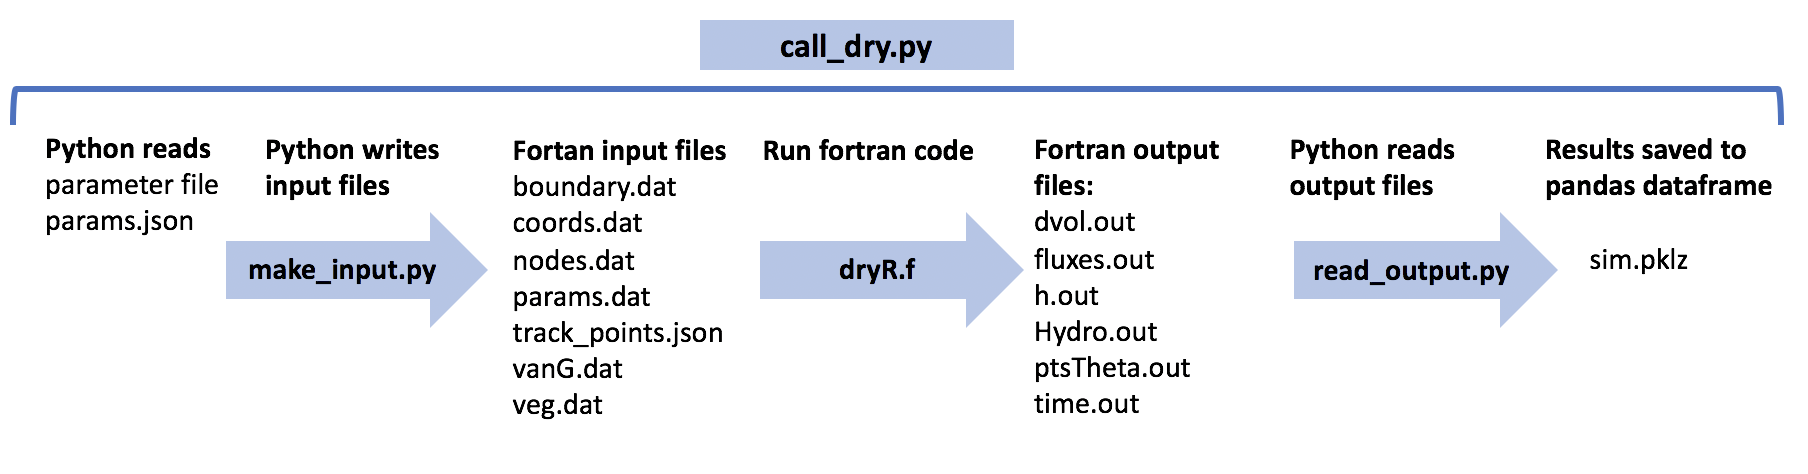
\includegraphics[width=38pc]{grid/schematic.png}
 \caption{Schematic illustrating the python wrapper script workflow. \code{call\_dry} takes as input \code{sim\_name}, the name of a subfolder containing the parameter file \code{params.json}.}
 \label{schematic}
 \end{figure}
 
 \code{call\_dry.py}  is a control script which writes the Fortan input files, compiles and executes the Fortran code dry.for, and reads the output files. 
It contains three main sub-functions, listed below:
 \begin{itemize}
		\item \code{sim\_input.py} 
		\item \code{runmodel}
		\item \code{sim\_read.py}
 \end{itemize}
 


 
\subsection{\code{sim\_input.py}: writes the Fortran input files}


\code{sim\_input.py} takes the input arguement \code{sim\_path}, the path to the simulation directory containing a parameter file \code{params.json}, and sets up the required file structure. This involves:
\begin{itemize}
	\item copying \code{dry.f} and \code{dry.inc} to \code{sim\_path};
	\item making \code{sim\_path/input} and \code{sim\_path/output} subdirectories;
	\item  reading and interpreting the parameter file \code{params.json}    
\end{itemize}   


\code{sim\_input.py} calls the following functions to write the input files (located in \code{sim\_name/input}):
\begin{itemize}
	\item \code{write\_param}: writes the general parameter file  \code{params.dat}.
	\item \code{input\_veg.py}: contains functions to write the input vegetation file \code{veg.dat}.
	\item \code{input\_coords.py}: contains functions to write the  grid and topography files \code{coords.dat}, \code{nodes.dat}. 
	\item \code{input\_boundary.py} contains functions to write the boundary file \code{boundary.dat}.
\end{itemize}

See appendix B for examples of the Fortran input files.

\subsubsection{\code{params.json}: specifies the parameters}
SVE parameters include:
\begin{itemize}
%%%%%%%%%%%%%%%%%%%%%%%%%  Grid setup. %%%%%%%%%%%%%%%%%%%%%%%%%
	\item \code{dx}: grid discretization (default = 1 m)  
	\item \code{nrow}:  number of grid cells in the along-slope direction.
		\subitem hillslope length \code{Ly} = \code{nrow * dx} 
	\item \code{ncol}:  number of grid cells in the across-slope direction (default = 10).
	 	\subitem hillslope width \code{Lx} = \code{ncol * dx} 
	\item \code{topo}: topography type (default = "plane", specifying a planar hillslope). 

	\item \code{vegtype}: specifies the vegetation field type, with options:
		\begin{itemize}
		\item \code{randv}: randomly-generated vegetation field, constructed with parameters $f_V$ (vegetation fraction) and $\sigma_x$, $\sigma_y$, (across- and along-slope patch length-scales).
	    \item \code{image}: read vegetation field from an image file (e.g. jpeg or png). In this case, the image file name must be included under the field \code{image\_name}.
		\end{itemize}
%%%% Resistance formualtion  
	\item \code{alpha} / $\alpha_V$: generalized roughness parameters for vegetated / permeable areas. If Manning's equation is used, then  $\alpha = n$.
	\item \code{alpha\_B} / $\alpha_B$: equivalent to \code{alpha} / $\alpha$   for bare soil areas.
%%%%%  Solver parameters 
	\item \code{epsh} / $\epsilon$: depth tolerance for dry cells.  The momentum equations are not solved if \code{h< epsh} ($h<\epsilon$).
	\item \code{beta} / $\beta$: a constant in limiter subroutine if ilim = 5, beta family (default = 1).   
\end{itemize}

Infiltration parameters include:
\begin{itemize}
	\item \code{Ks}: infiltration rate in vegetated/permeable areas, in cm/hr.  
	\item \code{KsB}: infiltration rate in bare soil/impermeable areas, in cm/hr.
	
	\item \code{stop\_tol}: error tolerance for Richards equation convergence,	default = 0.01

	\item \code{tsat\_min}: default = 600.  Specified in seconds.  Minimum time until the soil is allowed to saturate ($i$ is set to $K_{sat}$, bypassing the Richards equation solver
	\item \code{H\_i}: initial $H$ at the surface (the soil is initialized to an equilibrium profile).

	\item \code{tr}: storm duration (min)
	\item \code{p}: rain intensity (cm/hr)
\end{itemize}


\subsection{\code{runmodel}: compiles and execute \code{dry.f}}
The function \code{runmodel}, located in \code{call\_dry.py}, uses the Python os library to compile and execute \code{dry.f} with command line arguments: 

\begin{verbatim}
 os.system("gfortran -o {0}/sw  -framework accelerate {0}/dry.for".format(sim_path))
 os.system("cd {0} \n ./sw  \n cd {1}".format(sim_path, current_dir))	
\end{verbatim}

    
\subsection{\code{read\_sim}: reads the Fortran output files }

 \code{sim\_read.py} reads the output files and saves the results as a dictionary  \code{sim.pklz}.  The variables to be saved are lisrted\code{fortran\_outvars}.   \code{sim\_read.py}  executes the functions: 

\begin{itemize}
	\item \code{read\_time}: reads \code{time.out}
	\item \code{read\_hydro}: reads \code{hydro.out} and returns \code{t\_h} and \code{hydro}. The hydrograph is normalized by the hillslope dimensions to convert m$^3$/s to cm/s.
	\item \code{get\_h}: reads \code{h.out}, which contains the primitive variables (\code{h,u,v}), infiltration  (\code{inflVmap}), and the inter-cell fluxes \code{xflux0,yflux0,xflux1,yflux1}, all with dimensions: \code{nprt x ncol x nrow} (where \code{nprt} is the number of timesteps).
	\item \code{get\_dvol.py}: reads \code{dvol.out}, containing volume tracking variables  \code{vol},  \code{flux} and  \code{infl}, representing the total change in volume, lateral boundary fluxes and infiltration since the previous print timestep (i.e. \code{dt\_p}). \code{get\_dvol.py} normalizes by the domain area and converts to cm. 
\end{itemize}

 

	
\section{Select examples}	
\label{select_examples}

The following example simulations are included to demonstrate the model functionality, which can be used as templates:
\begin{itemize}
	\item \code{example\_2by2}: illustrate the grid set-up for a 2$\times$2 domain (see appendix B).
	\item  \code{example\_image}: rain driven overland flow on a planar hillslope with the vegetation field read from an image file.
	\item \code{example\_inflow} illustrates a subcritical inflow boundary at the top of the hillslope, with rain = 0 and $K_s=0$.
	\item \code{example\_rain}:  rain driven overland flow on a planar hillslope with the randomly-generated vegetation field.
\end{itemize}

Jupyter notebook files within each of these folders are included to visualize the simulated results.

Additionally, several template notebooks are included to process the SVE-R simulation results:

\begin{itemize}
	\item \code{example\_mass\_balance.ipynb}: Check mass balance in the SVE-R model. 
\end{itemize}

\section{Emulator feature code}
\label{emulator}
Code to generate the emulator features is provided in \code{feature\_functions.py}, with the Jupyter notebook \code{example\_features.ipynb} provided to interface with the results.
Within \code{RF\_patterns.py}, the  function \code{get\_feature\_matrix} takes an input binary (im)permeability pattern and returns a matrix of features, where each row corresponds to a grid cell in the input pattern.


 \begin{thebibliography}{}
 \bibitem{bradford1999hydrodynamics} Bradford, S. F., \& Katopodes, N. D. (1999). Hydrodynamics of turbid underflows. I: Formulation and numerical analysis. Journal of hydraulic engineering, 125(10), 1006-1015.

 \bibitem{bradford2001finite} Bradford, S. F., \& Katopodes, N. D. (2001). Finite volume model for nonlevel basin irrigation. Journal of irrigation and drainage engineering, 127(4), 216-223. https://doi.org/10.1061/(ASCE)0733-9437(2001)127:4(216)
 
 \bibitem{celia1990general} Celia, M. A., Bouloutas, E. T., \& Zarba, R. L. (1990). A general mass‐conservative numerical solution for the unsaturated flow equation. Water resources research, 26(7), 1483-1496.  https://doi.org/10.1029/WR026i007p01483

 \bibitem{pedregosa2011scikit} Pedregosa, F., Varoquaux, G., Gramfort, A., Michel, V., Thirion, B., Grisel, O., ... \& Vanderplas, J. (2011). Scikit-learn: Machine learning in Python. Journal of machine learning research, 12(Oct), 2825-2830.
 \end{thebibliography}


\appendix


\renewcommand\thefigure{A\arabic{figure}} 
\renewcommand\thetable{A\arabic{table}}
\setcounter{figure}{0}
\setcounter{table}{0}


\section{Relating \code{dry.f} code to the SVE and Richards equation }


The following is a partial list of grid correspondences:
\begin{itemize}
	\item $ U_\xi = \code{uxi} $
	\item $ U_\eta = \code{ueta}$
	\item  $d\xi$ = \code{dxi} 
	\begin{itemize}
		\item  $\xi_x = \code{dxi(1)} $
		\item  $\xi_y =\code{dxi(2)}  $
	\end{itemize}
	\item  $d\eta$ = \code{deta} 
	\begin{itemize}
		\item  $\eta_x = \code{deta(1)} $
		\item  $\eta_y =\code{deta(2)}  $
	\end{itemize}	
	\item  $\dfrac{dz}{dx}$= \code{sx}
	\item  $\dfrac{dz}{dy}$= \code{sy}
\end{itemize}
% Vertical cell faces have index 1, horizontal faces have index 2
% \code{ds(j,k,2)}: area of the lower horizontal boundary of cell \code{j,k} (\code{ipos = 1}), in m$^2$.

\subsection{The predictor step}

The \code{predict} subroutine is called for each cell to obtain \code{hp}, \code{up},  \code{vp} (corresponding to $h^{n+1/2}$,$u^{n+1/2}$,$v^{n+1/2}$).   \code{predict}  modifies the common variables  \code{hp}, \code{up},  \code{vp}, \code{dh}, \code{du}, \code{dv}, \code{qs}.


The following provides an (incomplete) correspondence between BK equations and Fortran code, with the mathematical notation in \textit{italics} and the equivalent code in \code{typewriter}.   For example, for the array of primitive variables:
\[  \mathbf{W_T} = 
\begin{bmatrix}
	h \\
	U \\
	V \\
\end{bmatrix}
 =  {
	 \begin{bmatrix}
	 \code{h} \\
	 \code{u} \\	 
	 \code{v} \\	 	 	 
\end{bmatrix} 
}  \]


The matrices $\mathbf{A}_W$ and $\mathbf{B}_W$ are defined as: 

\[ \mathbf{A}_w = 
\begin{bmatrix}
    U_{\xi} & h \xi_x & h \xi_{y} \\
    g \xi_x &    U_{\xi}  & 0    \\
    g \xi_y &   0   & U_{\xi}    \\    
\end{bmatrix} =
\begin{bmatrix}
    \code{uxi }& \code{h} \ \code{dxi(1)} &\code{h*dxi(2)}\\
    \code{g dxi(1)}& \code{uxi} & 0  \\    
    \code{g dxi(2)}&     0       & \code{uxi}  \\          
\end{bmatrix} 
\]

\[ \mathbf{B}_w = 
\begin{bmatrix}
    U_{\eta} & h \eta_x    & h \eta_{y} \\
    g \eta_x &    U_{\eta}  & 0    \\
    g \eta_y &      0       & U_{\eta}    \\    
\end{bmatrix} =
\begin{bmatrix}
    \code{ueta }  & \code{h*deta(1) } & \code{h*deta(2)}\\
    \code{g dxi(1)} & \code{ueta}  & 0  \\    
    \code{g dxi(2)} &     0  	   &  \code{ueta}  \\          
\end{bmatrix} 
\]


\[ \partial_\xi \mathbf{W} = 
\begin{bmatrix}
    \partial_\xi h \\
	\partial_\xi u \\
    \partial_\xi v \\
\end{bmatrix}
 =  {
	 \begin{bmatrix}
	 \code{dh(1)} \\
	 \code{du(1)} \\	 
	 \code{dv(1)} \\	 	 	 
\end{bmatrix} 
}  ;  \quad  \quad
\partial_\eta \mathbf{W} = 
\begin{bmatrix}
    \partial_\eta h \\
	\partial_\eta u \\
    \partial_\eta v \\
\end{bmatrix}
 =  {
	 \begin{bmatrix}
	 \code{dh(2)} \\
	 \code{du(2)} \\	 
	 \code{dv(2)} \\	 	 	 
\end{bmatrix} 
}
 \] 


where  \code{dh(1)} implies \code{dh(j,k,1)}, and similarly for  \code{du(1)} and  \code{dv(1)}. 

$ \mathbf{A}_w \partial_\xi \mathbf{W} $ is computed as:

\[ \mathbf{A}_w \partial_\xi \mathbf{W} = 
\begin{bmatrix}
    U_{\xi} & h \xi_x & h \xi_{y}  \\
    g \xi_x &    U_{\xi}  & 0   \\
    g \xi_y &   0   & U_{\xi}    \\           
\end{bmatrix} 
\begin{bmatrix}
    \partial_\xi h \\
	\partial_\xi u \\
    \partial_\xi v \\
\end{bmatrix}
 =  
	 \begin{bmatrix}
	  U_{\xi}  \partial_\xi h +  h \xi_x  \partial_\xi u + h \xi_{y} \partial_\xi v \\[.1cm]
	  g \xi_x \partial_\xi h  +  U_{\xi} \partial_\xi u    \\[.1cm]
	  g \xi_y  \partial_\xi h  +  U_{\xi}  \partial_\xi v  \\	 	 
\end{bmatrix} 
 \]

Equivalently in code:

\begin{equation*}\label{theta-alt}
\begin{aligned}
\mathbf{A}_w \partial_\xi \mathbf{W}  &=
 \begin{bmatrix}
     \code{uxi} & \code{h dxi(1)} & \code{h  dxi(2) } \\
     \code{g dxi(1)} & \code{uxi} &  0  \\     
     \code{g dxi(2)} & 0 &  \code{uxi}  \\     
\end{bmatrix}
	 \begin{bmatrix}
	 \code{dh(1)} \\
	 \code{du(1)} \\	 
	 \code{dv(1)} \\	 	  	 	 
\end{bmatrix}  = \\
&\qquad\qquad
	 \begin{bmatrix}
	  \code{uxi*dh(1) + h*(dxi(1)*du(1) + dxi(2)*dv(1))} \\
	   \code{g*dxi(1)*dh(1)  + uxi*du(1) } \\ 	 	 	 	 
	   \code{g*dxi(2)*dh(1)  + uxi*du(1) } \\ 	 	 	 	 	   
\end{bmatrix} 
\end{aligned}
\end{equation*}



The \code{limitr} subroutine contains the flux limiter that the predictor step uses to compute the cell-average spatial gradients (which preserves solution monotonicity by becoming first-order accurate near discontinuities, yet remains second-order accurate elsewhere).
Various choices are included, with the parameter \code{ilim} specifying the averaging type. \code{ilim}=5 instructs the code to use the $\beta$ family of averages, and is given by:

\begin{eqnarray*}
	\mathbf{\overline{\Delta W}} = \text{sign}(a)\text{min}[\text{max}(|a|, |b|), \beta(|a|, |b|)]  \textmd{  if }  ab>0  \\ 
	0 \textmd{ if }  ab \leq 0	
\end{eqnarray*}

$\beta$ = 1 yields the relatively more dissipative Minmod average, and $\beta $ = 2 yields the less dissipative Superbee average. 


\subsection{The corrector step}

The corrector step computes the fluxes between the cell interfaces by calling the \code{fluxes} subroutine for each cell \code{j,k} and for each interface. 

The interfacial cell fluxes at a given time-step are stored in the common variable \code{f(0:nx,0:ny,1:3,1:2)}, where the first two indices of \code{f} contain the $j,k$ coordinates, the third index correspond to the components of  $\mathbf{F_\perp}$ (see Equation), and the final index denotes the cell face (1 for vertical cell faces and 2 for horizontal).   
\code{f(j,k,1:3,1)} represents the flux from cell $(j-1, k)$ to $(j, k)$, and
\code{f(j,k,1:3,2)} represents the flux from cell $(j, k-1)$ to $(j, k)$ (see Figure \ref{fluxes_specific_A}).
Calling \code{fluxes(j-1,j,k,k,1)} modifies \code{f(j,k,1:3,1)}  and calling \code{fluxes(j,j,k-1,k,2)} modifies \code{f(j,k,1:3,2)}.

 \begin{figure}[h]
 \centering
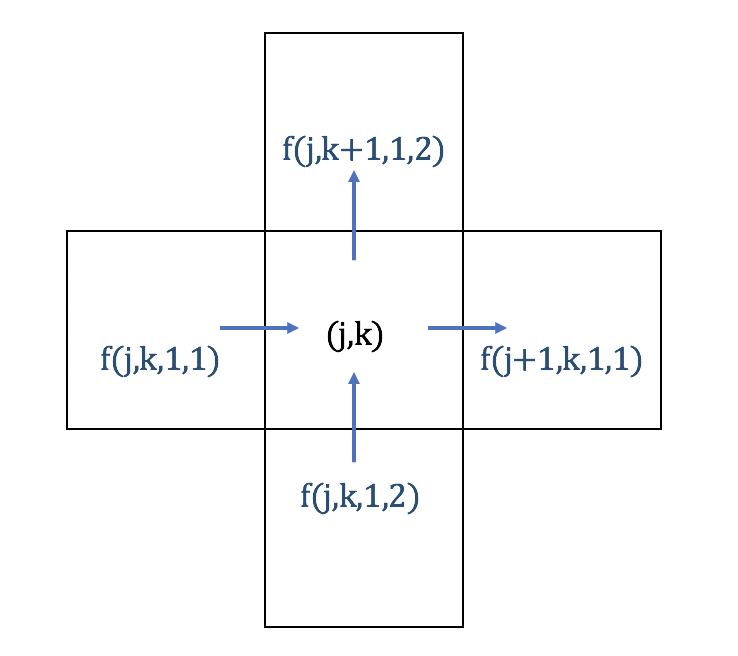
\includegraphics[width=15pc]{grid/fluxes_specific.png}
 \caption{Definitional sketch for the interfacial fluxes, indicating how the fluxes into and out of cell (j,k) are stored in the array \code{f(0:nx,0:ny,1:3,1:2)}}.
 \label{fluxes_specific_A}
 \end{figure}

\subsubsection*{Fluxes subroutine}

Within the \code{fluxes} subroutine, \code{fluxes(jl,jr,kl,kr,i1)} computes the flux from cell \code{(jl,kl)} to \code{(jr,kr)}, modifying the common variable \code{f(jr,kr,1:3,i1)}. 
\code{i1 = 1} indicates that the flux is between vertical cell faces, i.e. from cell \code{(j-1,k)} to \code{(j,k)}.
Similarly, \code{i1 = 2} indicates that the flux is between horizontal cell faces, i.e. from cell \code{(j,k-1)} to \code{(j,k)}.

 
\code{fluxes}  first reconstructs the predicted values to the left and right of each face (\code{hl,hr,ul, ur,vl,vr)} using the monotone upstream scheme for conservation laws (MUSCL).  These reconstructed predictor values define a Riemann problem at each cell face, and \code{fluxes} calls the \code{solver} subroutine to compute $\mathbf{F_{\perp I}}$ from BK1999 Equation 27:

\begin{equation}
\mathbf{F_{\perp I}} =
	 \frac{1}{2} (\mathbf{F_{\perp L}} + \mathbf{F_{\perp R}} - \mathbf{\hat{R} |\hat{\Lambda}| \Delta \hat V  })
	 \label{BK27}
\end{equation}

%% equations from BK are reproduced here in order to relate these equations to  the Fortran code.t

\subsubsection*{The solver subroutine}

This subroutine uses the monotone upstream scheme for conservation laws (MUSCL) to compute $\mathbf{F_\perp}$ at each cell face.  The code in \code{solver} corresponds to BK1999 Equation 27 as: 

 \begin{itemize}
 	\item $\mathbf{\hat{R}}$: \code{e(3,3)}
 	\item $\mathbf{|\hat{\Lambda}|}$: \code{a(3) }
 	\item $\mathbf{\Delta \hat V  }  $: \code{ws(3)} 
 \end{itemize}
 
 \[ \mathbf{\hat{R}} = 
\begin{bmatrix}
    1 &  0  & 1  \\
    \hat{u} -\hat{a} \cos{\phi} &   -\sin{\phi} & \hat{u} +\hat{a} \cos{\phi}   \\
    \hat{v} -\hat{a} \sin{\phi} &   \cos{\phi} & \hat{v} +\hat{a} \sin{\phi}    \\
\end{bmatrix} = 
\begin{bmatrix}
    1 &  0  & 1  \\
    \code{uhat-chat*cndum} &    \code{-sndum} &  \code{uhat+chat*cndum} \\
    \code{vhat-chat*sndum} &    \code{cndum} &  \code{vhat+chat*sndum} \\
\end{bmatrix}
\]

\
 
 \[ \mathbf{|\hat{\Lambda}|} = 
\begin{bmatrix}
  |\hat{u}_\perp - \hat a| &  &  \\
     &   |\hat{u}_\perp | &  \\ 
     & &  |\hat{u}_\perp  + \hat a| \\
\end{bmatrix} \ =  \
\begin{bmatrix}
 \code{|uperp - chat|} &  &  \\
     &    \code{|uperp |} &  \\ 
     & &   \code{|uperp + chat|} \\
\end{bmatrix} 
\]


 \[ \mathbf{\Delta \hat{V}} = 
\begin{bmatrix}
	\frac{1}{2} \bigg( \Delta h - \dfrac{\hat h \Delta u_{\perp} }{\hat a} +
	 \dfrac{\hat h \Delta c_T }{2  c_T}\bigg) \\[.2cm]
      \hat h \Delta u_\parallel   \\[.2cm]
   	\frac{1}{2} \bigg( \Delta h + \dfrac{\hat h \Delta u_{\perp} }{\hat a} +
	 \dfrac{\hat h \Delta c_T }{2  c_T}\bigg) 
	 \\
\end{bmatrix} \ =  \ 
\begin{bmatrix}
 \code{0.5*(dhdum - hhat*duperp/chat)}  \\[.2cm]
 \code{hhat*dupar}  \\[.2cm]
 \code{0.5*(dhdum - hhat*duperp/chat)}  \\
\end{bmatrix} 
\]

  \begin{itemize}
 	\item  $\Delta h$: \code{dhdum = hr - hl } 
 	\item  Left interface:   \code{hl = hp(jl,kl) + 0.5*dh(i1)}
  	\item  Right interface:   \code{hr = hp(jl,kl) - 0.5*dh(i1)}
	 \item Interface number: \code{i1} 
 \end{itemize}
 

\subsection{The source subroutine}

% Infiltration and surface resistance are represented in 
 The source term is computed with the subroutine \code{source}, which modifies the common variable \code{qs} (or $Q(j,k)$).
  \code{source} is called by both the predictor and corrector steps; however, Richards equation is only solved during corrector step. 
 The input arguments are the  cell indices \code{j,k}, the primitive variables, and \code{lstep} (an indicator variable for the step type: \code{lstep = 0} for the predictor step and \code{lstep = 1}  for the corrector step).	
 
In the predictor step, \code{source} is called for each cell before updating the predictor values (\code{hp,up,vp}):
\begin{center}
\code{call source(j, k, h(j,k), u(j,k), v(j,k), 0)}
\end{center}

 
\code{source} is similarly  called in the corrector step before updating the fluxes: 
\begin{center}
\code{call source(j, k, hp(j,k), up(j,k), v[(j,k), 0)}
\end{center}

Inside \code{source}, the primitive variables are labeled \code{depth,udum,vdum}. 
The source term in Fortran code is given as:

\[ \mathbf{Q} = 
 \begin{bmatrix}
	\code{winflt}  \\[.1cm]
	\code{-grav*depth*sx(j,k)-grav*depth*fricSx+0.5*udum*winflt}\\[.1cm]
	\code{-grav*depth*sy(j,k)-grav*depth*fricSy+0.5*vdum*winflt}\\[.1cm]
\end{bmatrix} 
\]

where $S_{f,x}$ = \code{fricSx} and  $S_{f,x}$ = \code{fricSy}, and $p-i$ = \code{winflt}.


\subsubsection*{Infiltration details (corrector-step)}

In the corrector step, \code{source} calls the infiltration-specific subroutines (\code{timestep} and \code{potential} to update the infiltration rate $i$ and the surface boundary conditions at cell \code{j,k}. 
%calls th subroutines (\code{potential} and \code{timestep}) to solve Richards equation. 
\code{timestep} solves Richards equation at cell \code{(j,k)} and returns the updated $H$, $\theta$ and $K$, which \code{source} uses to compute the infiltration rate $i$. \code{potential} is used to prescribe the boundary conditions. 

 The Richards equation solver is implemented separately for each grid cell, and the 3-dimensional $H$, $\theta$ and $K$  fields are saved as the common variables \code{r8H} (cm), \code{r8Theta}, and  \code{r8K} (cm/s), respectively, with dimensions (\code{nrow} $\times$ \code{ncol} $\times$ \code{nz}).\\ 

%%%% ADD POTENTIAL INFILTRATION

\noindent From Darcy's law, the infiltration rate $i$ (cm/s) is computed as:
$$ i =  K \bigg(\frac{\partial H}{\partial z} + 1\bigg ) $$
which corresponds to \code{r8kt*((hdum(nz)-hdum(nz-1))/dz+1)} in \code{source}.

\noindent  As an intermediate step, the depth is updated with: \\
\begin{center}
\code{znew=  zold + rain*100*dt - r8kt*( (hdum(nz) - hdum(nz-1))/dz + 1)*dt } 	
\end{center}
where \code{rain}  rainfall has been converted to cm/s.
 \code{winflt} = $p-i$  is then computed as:
\begin{center}
 \code{winflt = (znew - zold)/dt/100.} 	
\end{center}

%Note that \code{znew} is computed as a separate step for code readability, and things could be simplified to: \code{winflt = rain*100 - r8kt*( (hdum(nz) - hdum(nz-1))/dz + 1)} .
	
 

\subsection{The Richards equation subroutine (\code{timestep}) }

Richards equation is solved by the \code{timestep} subroutine, which is called from \code{source}.
	
\subsubsection*{\code{timestep} inputs and outputs }
The inputs are \code{hnp1m} and \code{thetan}, which are the initial conditions to the Richards equation solver (\code{hdum,thetadum} in the source subroutine).  
The outputs are  \code{hnp1mp1,r8thetanp1m,r8knp1mp1}, which are  $H$, $\theta$ and $K$ at the following timestep (after \code{dt\_r}  time elapsed).


%$ i =  K (\frac{\partial H}{\partial z} + 1) $, which corresponds in the Fortran code to \code{r8kt*( (hdum(nz) - hdum(nz-1))/dz + 1)}. 

When the soil is flagged as too homogenous for matrix inversion (i.e. `saturated'),  the surface flux is set to $K$ at the surface, which will be approximately saturated if $p > K_{sat}$ (\code{flux  = - r8knp1m(nz)}).  

\subsubsection*{Stop tolerance }
\code{stop\_tol0} is the stop tolerance specified in the input \code{params.dat}, with default value \code{stop\_tol0 = .01}.  
\code{stop\_tol} is reset to the original \code{stop\_tol0}  at the beginning of each Richards solver timestep.  The convergence tolerance  is relaxed if the Richards solver fails to converge within a specified number of iterations (default = 100).



\subsubsection*{Potential infiltration}

The subroutine \code{potential} is used to compute the potential infiltration rate $PI$, defined as the infiltration that would be observed for a surface boundary condition of $H=0$. 
Potential infiltration is computed when there is rain but no ponding, and returns the potential infiltration rate, defined as the infiltration rate that would occur with $H=0$ at the surface.  



%\subsection{Source subroutine variables}
%
%\begin{itemize}
%	\item \code{isetflux} (common) specifies the boundary condition for the Richards equation solver.  \\[.2cm]
%	 \code{isetflux} = 1 if the surface flux is specified: \code{flux = 0} in case 3 (no rain and no ponding), and \code{flux = rain} in case 2 (rain and no ponding).\\[.2cm]
%	 \code{isetflux} = 0 if the surface H is specified (Dirichlet). If there is ponding (case 4), the surface boundary condition is $H$=$h$. 
%	\item \code{flux} is the surface flux (cm/s).  \code{flux} is a common variable defined in \code{source}, and used by \code{timestep}  if \code{isetflux=1}. 
%
%	\item \code{htop}: Upper boundary condition for fixed $H$ boundary condition (\code{isetflux=1}).
%
%	\item \code{PI} Potential infiltration, computed by the \code{potential} subroutine.
%
%	\item \code{depth, udum, vdum}: $h$, $U$, $V$ at grid cell \code{j,k}.
%		\subitem  \code{hp(j,k),up(j,k),vp(j,k)} if called from the corrector step.
%		\subitem  \code{h(j,k),u(j,k),v(j,k)} if called from the predictor step.	
%	\item \code{lstep} indicates from which sstep the source subroutine was called.
%		\subitem  \code{lstep} = 0 if called from the predictor step
%		\subitem  \code{lstep} = 1 if called from the corrector step. \\[.2cm]	
%		Infiltration is only updated depth in corrector step.
%		
%	\item \code{zold, znew}	: depth in cm  \\[.2cm]
%	 Richards solver units are in cm, whereas SVE-R solver units are in m)
%	\item \code{fm, feta, falpha}: roughness parameters $m$, $\eta$, and $\alpha$.
%\end{itemize}
%

\section{Input and output files, illustrated with a 2$\times$2 grid}



%\code{nop(1,1,:) = [1,4,5,2]} means that cell (1,1) is bounded by nodes \code{n1=1,n2=4,n3=5,n4=2}, starting from the lower left node \code{n1} moving counterclockwise.
% \code{itype(j,k,2)=1, itype(j,k,3)=4}, means that cell \code{(j,k)} has a closed boundary at position 2 (right) and a subcritical influx boundary at position 3 (top). See Figure	 \ref{nodes}.			
%	
	 

To illustrate the grid set-up, example input files are included here for the 2x2 grid example.  Note that while the SVE-R model Fortran code does not assume a  rectangular grid, the provided Python code and sample input files do assume a rectangular grid. 
 Figure \ref{2by2} shows the cell center and node indices for the example grid, and Figure \ref{2by2boundary} shows the boundaries, which are a fixed-flux subcritical boundary at the top of the hill, closed/wall lateral boundaries, and an open boundary at the bottom of the hill.


 \begin{figure}[h]
 \centering
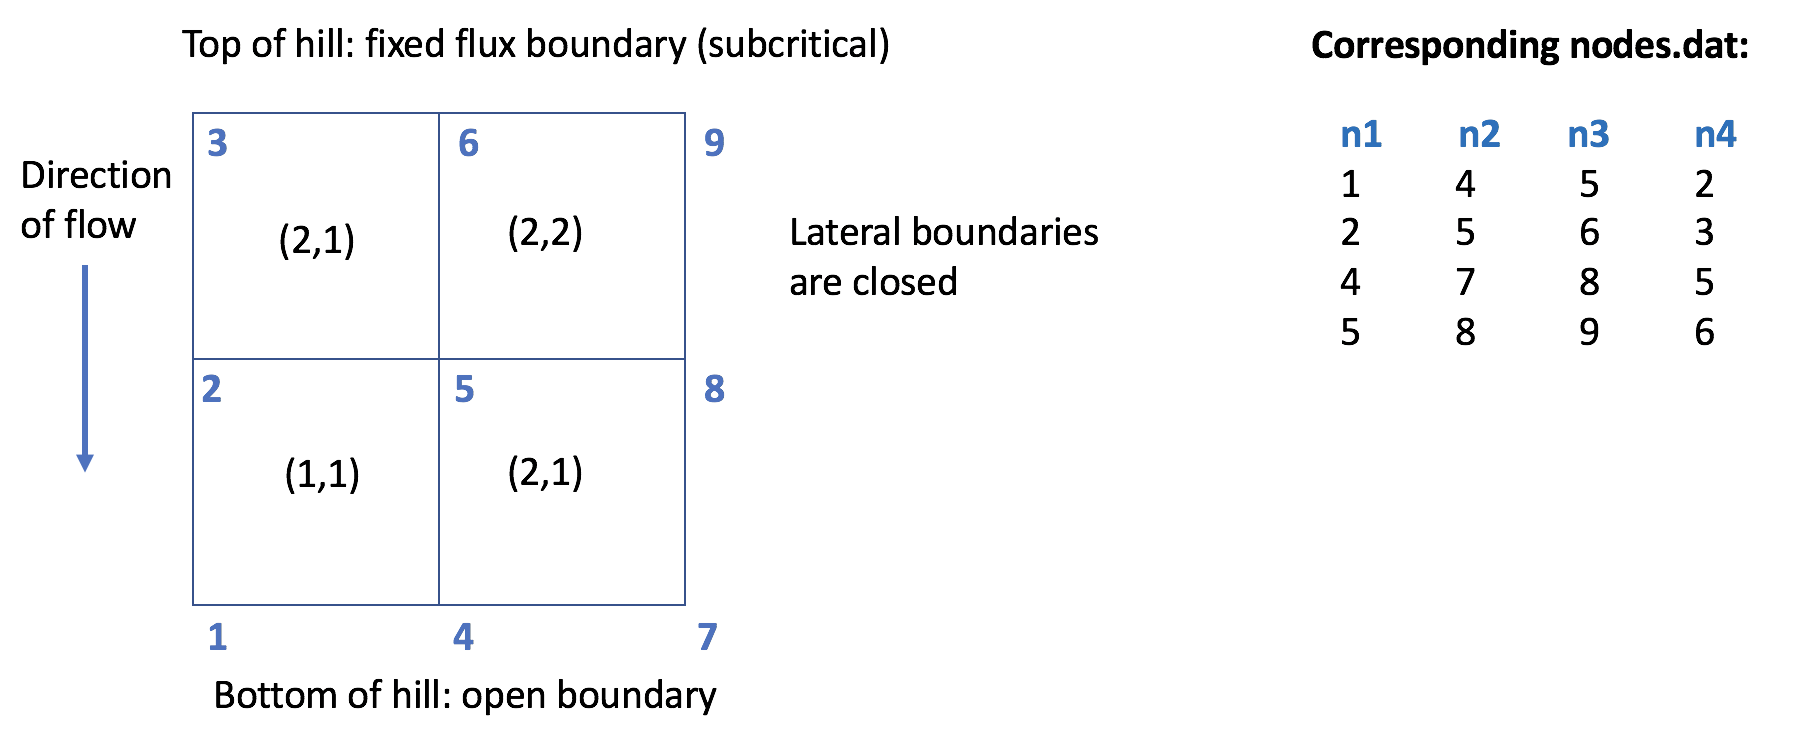
\includegraphics[width=30pc]{grid/2by2nodes.png}
 \caption{Example 2$\times$2 grid to illustrate how cell centers and nodes are assigned.  (j,k) coordinates are shown in the cell centers, and the node indices are at the cell corners. }
 \label{2by2}
 \end{figure}
 
 \begin{figure}[h]
 \centering
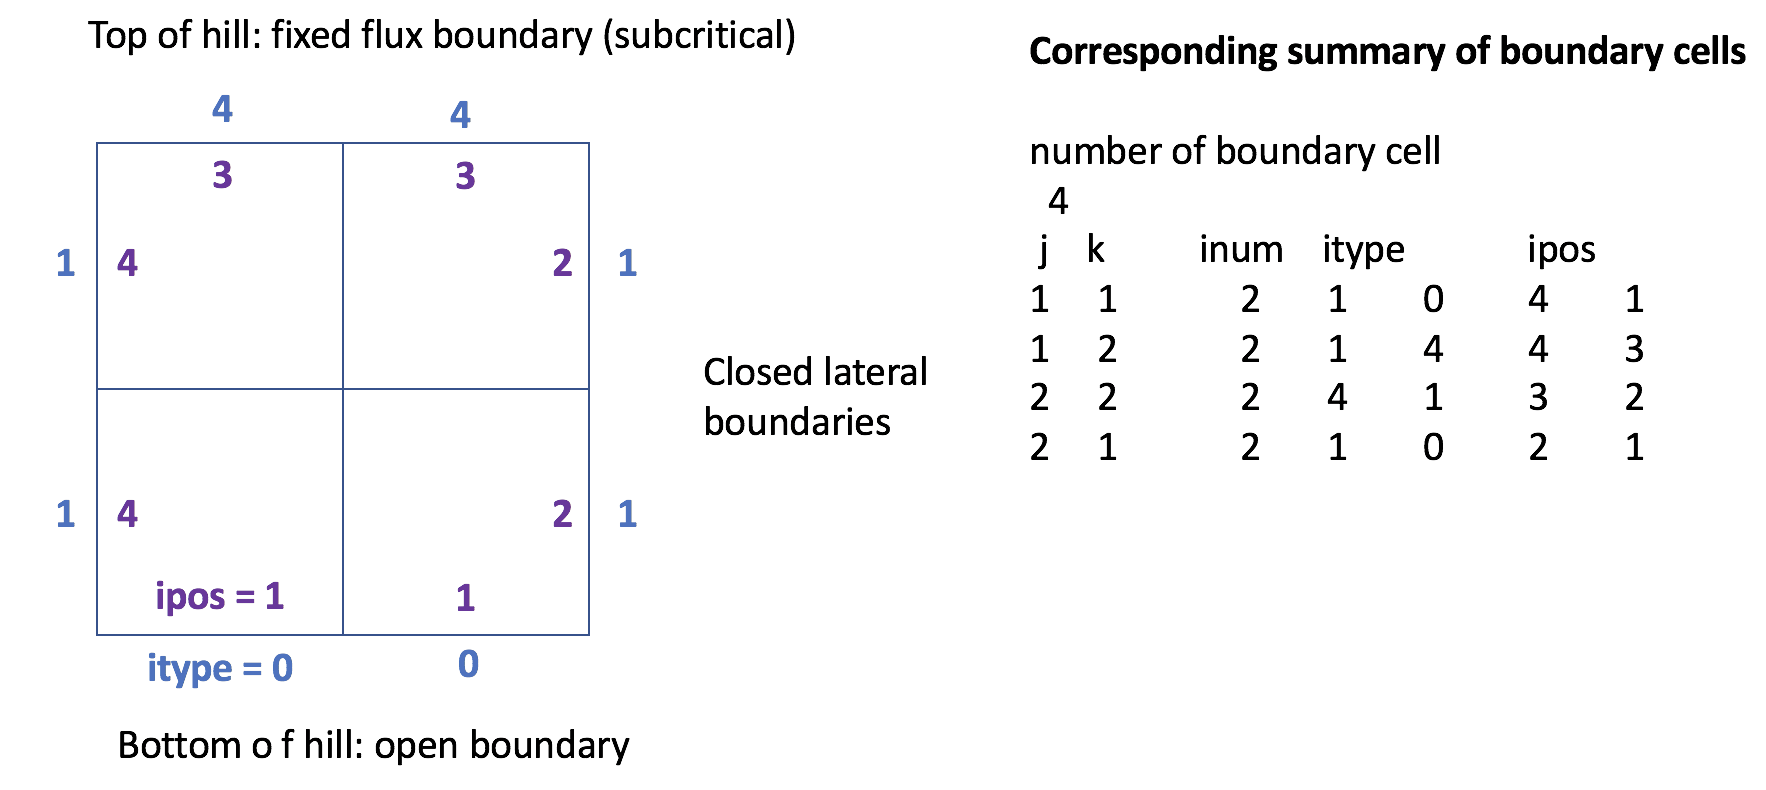
\includegraphics[width=30pc]{grid/2by2boundary.png}
 \caption{Boundaries for the 2$\times$2 grid in Figure \ref{2by2boundary}. The boundary types are labeled in blue outside the grid, with 0 for the open boundary, 1 for the closed boundaries and 4 for the fixed flux boundary.  }
 \label{2by2boundary}
 \end{figure}
 
\subsection{params.dat}

Sample \code{params.dat} files can be found in the \code{input} directories of the examples.  The parameters specified in \code{params.dat} are:
  
\begin{itemize}
	\item \code{grav}: acceleration due to gravity.
	\item \code{dt}: SVE timestep (\code{dt} is labeled \code{dt\_sw} in the Python code). 
	\item \code{tmax}: maximum time until the simulation ends.
	\item \code{tr}: rain duration in seconds (\code{tr} is labeled \code{t\_rain} in the Python code). 
	\item \code{rain}: rain intensity in m/s.
	\item \code{nt}:  number of time steps  (\code{tmax/dt})
	\item \code{epsh}: depth threshold to solve the SVE momentum equations.
	\item \code{beta}: value of beta in limitr subroutine.
	\item \code{nprt}: frequency f which the SVE-R output fields are saved: \code{nprt= dt\_p}.  Note: the hydrograph is saved every second.
	\item \code{iscale}: ratio of SVE to Richards equation timestep durations.
	\item \code{stop\_tol}: convergence criteria for Richards equation solver (default = 0.01).
	\item \code{h0, u0, v0}: initial depth, \code{u}, and \code{v} (defaults = 0).
	\item \code{r8mV,r8etaV, r8alphaV}: roughness parameters $m$, $\eta$ and $\alpha$ for vegetated cells. 
	\item \code{r8mB,r8etaB, r8alphaB}: roughness parameters $m$, $\eta$ and $\alpha$ for bare cells. 
	\item \code{jveg, kveg}: \code{j, k} indices of a vegetated cell for which the soil profile ($H$ and $\theta$) is saved every \code{nprt} timesteps.
	\item \code{jbare, kbare}: \code{j, k} indices of a bare soil cell for which the soil profile ($H$ and $\theta$) is saved every \code{nprt} timesteps.
	\item \code{tsat\_min}: Minimum time until the soil is allowed to ``sarturate'' (default =0).
\end{itemize}



 
% Following this, 
% the following rows record: 
% the number of columns and rows, and, for each column, 
% the beginning and final row  (i.e. \code{kbeg = 1} and \code{kend = nrow}.
%  
\subsection{boundary.dat}

\code{boundary.dat} specifies the boundary cell locations, types and orientations.  
For each boundary cell location (\code{j,k} indices), the number of boundary faces (\code{inum}), types (\code{itype}) and orientations (\code{ipos}) must be specified.
\code{boundary.dat} also lists any fixed boundary condition cells (\code{fix}) and the relevant primitive variables ($h$, $U$ and/or $V$, depending on the boundary type).

Provided boundary types are:
\begin{itemize}
	\item  \code{itype} = 1 for a closed boundary
	\item  \code{itype} = 0 for an open boundary
	\item  \code{itype} = 4 for 	 a subcritical inflow boundary
	\item  \code{itype} = 5 for a supercritical influx boundary
 \end{itemize}
 
For a subcritical inflow boundary,  the normal depth is computed  with Manning's equation with $n=0.1$.  
The input parameter \code{influx} is specified in unis m$^2$/s, which can be related to the rainfall rate (in cm/hr) as: $p$ = $q\cdot 3.6e5/L_y $ (cm/hr), or  \code{influx}  $q = p\cdot L_y/3.6e5$  (m$^2$/s).


Below is a sample \code{boundary.dat} for the 2x2 grid example, for which every cell is a boundary cell. 
The first two rows contain the number of boundary cells, defined as a grid cell with one or more boundaries.
The array on lines 3-7 show the (j,k) indices for each boundary cell, the number of boundaries associated with that cell, and boundary type of each boundary cell.

\begin{verbatim}
number of boundary cell 
  4 
 j    k          inum    itype             ipos 
1     1             2       1        0         4        1      
1     2             2       1        4         4        3      
2     2             2       4        1         3        2      
2     1             2       1        0         2        1      
ncol
2
nrow
2
j     kbeg          kend 
    1      1             2   
    2      1             2   
number of fixed bc cells, ndir    
 2  
 j     k    fix h    fix u    fix v	
1     2     0.0     0.0     -2e-05     
2     2     0.0     0.0     -2e-05     
\end{verbatim}

\subsection{coords.dat}

In the two rows specify the number of nodes (\code{npt}) and the number of cells (\code{ne}).  The remaining rows list the x,y,z coordinates at the nodes, in order of node number. Below is an example \code{coords.dat} file for the 2$\times$2 exampleg rid.


\begin{verbatim}
npt             ne           
9               4            
x             y             z              
0.00          0.00          0.00           
0.00          1.00          0.02           
0.00          2.00          0.04           
1.00          0.00          0.00           
1.00          1.00          0.02           
1.00          2.00          0.04           
2.00          0.00          0.00           
2.00          1.00          0.02           
2.00          2.00          0.04           
\end{verbatim}

\subsection{vanG.dat}

\code{vanG.dat} specifies the soil dimensions, van Genuchten parameters and initial $H$ profile, independently for vegetated and bare soil cells (Note: all vegetated cells have the same parameters and ICs, and likewise for the bare soil cells).   See example below from the 2$\times$2 grid example.
The first two rows specify the soil depth (\code{zmax}) and soil layer thickness (\code{dz}), and the second two rows specify the number of soil grid points (soil layers + 1).   
Following this, the soil parameters and initial $H$ for the vegetated cells are listed for each soil layer in order of decreasing soil depth (the first row is the lowest layer of the soil column).   This format is repeated for the bare soil cells.   
From left to right, the columns are: 
	$\alpha$,$\theta_S$,$\theta_R$, $\lambda$, $K_s$, $H_i$, where $\lambda =  n-1 $ in Equation \ref{vanG_eqn} and $H_i$ is initialize with an equilibrium soil moisture profile.
	
\begin{verbatim}
dz           zmax 
1.0           20             
nz 
21             
vegetated cells  
alpha    theta_S   theta_R    lambda    Ksat                   h_init 
0.0096   0.472     0.0378     0.47      0.000555555555556      -320.0 
0.0096   0.472     0.0378     0.47      0.000555555555556      -321.0 
0.0096   0.472     0.0378     0.47      0.000555555555556      -322.0 
0.0096   0.472     0.0378     0.47      0.000555555555556      -323.0 
						....
 bare soil cells 
alpha    theta_S   theta_R    lambda    Ksat                   h_init 
0.0096   0.472     0.0378     0.47      0.000555555555556      -320.0 
0.0096   0.472     0.0378     0.47      0.000555555555556      -321.0 
0.0096   0.472     0.0378     0.47      0.000555555555556      -322.0 
\end{verbatim}


\subsection{h.dat}

\code{h.out}: columns are \code{j,k,h,u,v,zinflmap2, xflux0,yflux0,xflux1,yflux1}. 
These variables are written for every grid cell, every \code{nprt} timesteps (i.e. at time intervals of \code{dt\_p}). Following this, the print iteration \code{itp} and current time {t} is written on a new line. An example for a 2$\times$2 grid is shown in Figure \ref{h.out_example}.  

 \begin{figure}[h]
 \centering
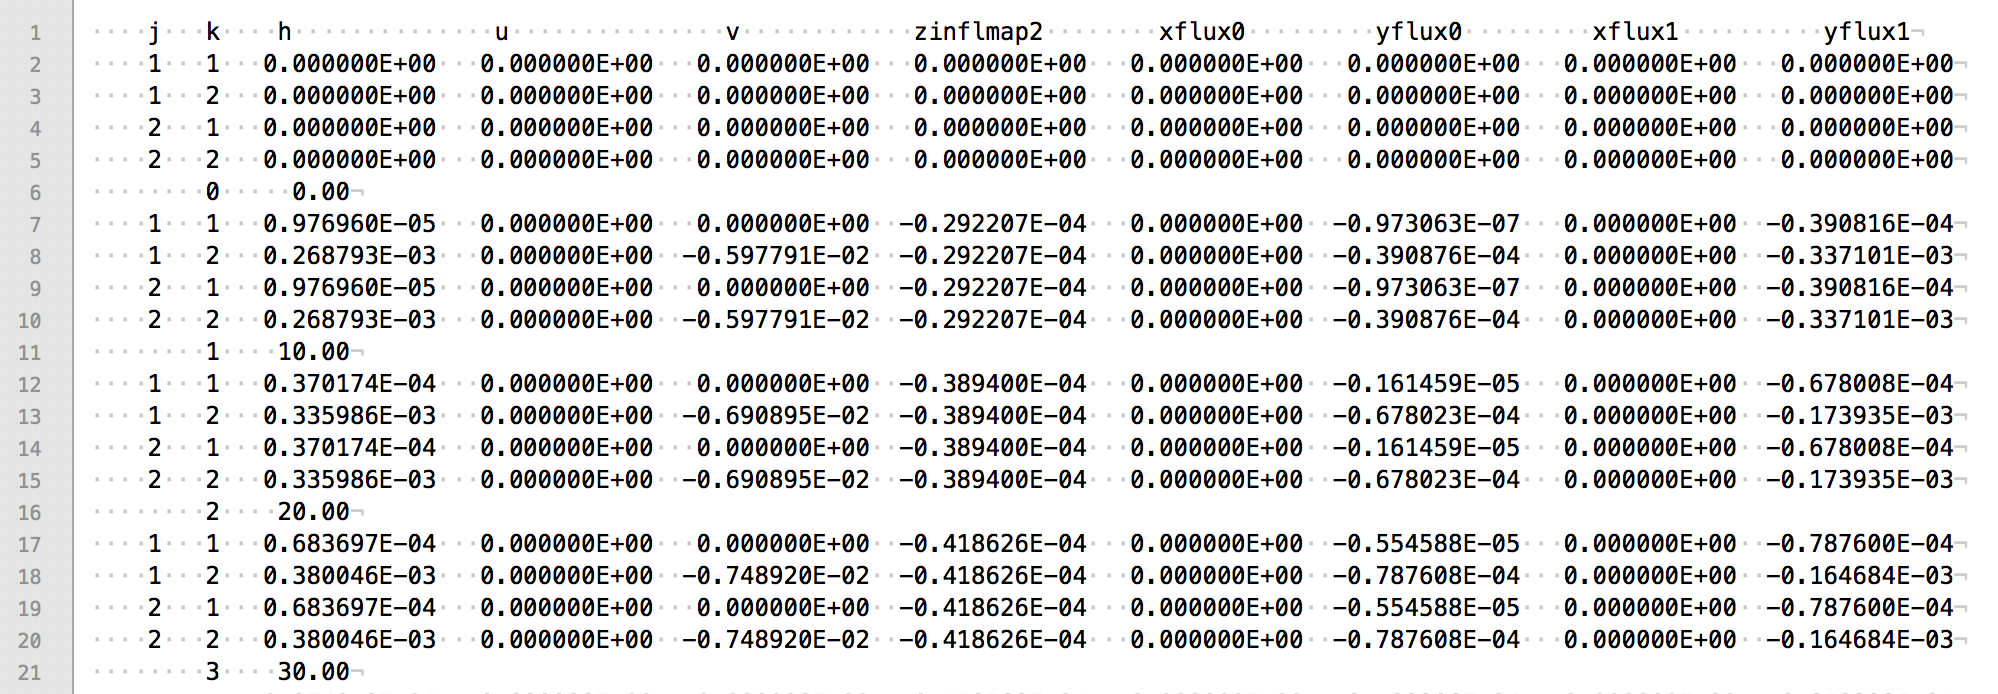
\includegraphics[width=35pc]{grid/h_out.png}
 \caption{Screenshot of a sample \	code{h.out} file.}
 \label{h.out_example}
 \end{figure}
  
  
% \code{zinflmap2} contains the total volume of water infiltrated in cell j,k, and is reset to zero when this variable is written to file. 


\subsection{dvol.dat}

Contains output from Fortran mass balance tracking.
Columns are \code{dvol, flux, infl} containing the  change in surface volume, horizontal fluxes out of the domain, infiltration and rain volumes, respectively, in units m$^3$.


%\subsubsection*{hydro.out}




\section{\code{dry.f} pseudocode}

\subsection{Model overview/summary}

\begin{lstlisting}
 
call init ! grid  subroutine called from the input subroutine
call myoutput  !  write initial conditions to file


do it = 0,nt-1   ! loop over time steps (it = time iteration number)
	t = t+dt   ! increment time (t = current time)

	! Predictor step
	loop over grid cells: 
		call bconds(j, k, h, u, v)    ! update h,u,v values in ghost cells
		call predict(j, k)            ! get predictor variables hp, up, vp

    ! Corrector step
	! Corrector part 1: compute the fluxes between cell faces
	loop over grid cells: 			  
    call bconds(j,k,hp,up,vp) ! update hp,up,vp in the ghost cells
    ! compute interfacial fluxes. 
    call fluxes(j-1,j,k,k,1)      ! vertical faces. 
    call fluxes(j,j,k-1,k,2)      ! horizontal faces.
	loop over boundaries:
		compute boundary fluxes
	
	! Corrector part 2: 
	loop over cells:
		call source ! update the source term qs
		compute q from qs and f	! q = (h,uh,vh)
		! update h,u,v from q. check 
	    if q > 0:				! check for negative depth.	
			h = q(1) 		    ! if positive depth, update h
	    else:
			q = 0 				! if negative depth, reset h and q(1) to zero
			h = 0					  
	
	    if h < epsh: 		!  neglect momentum in nearly dry cells
			u, v = 0.		!  set u and v to 0 in nearly dry cell	  
			q(2:3) = 0 		!  set momentum fluxes to 0
	    
	    elif h >= epsh:		!  store u and v values
	    	u, v = q(2)/h, q(3)/h
		    
    ! Exit when the ponded water is less than min_vol    
    if volume < min_vol
    	call gracefulExit
    	
    ! Exit when the CFL number is too big
    if(CFL > 10) then
        call gracefulExit
        
	! Exit if time runs out
    if(t > tmax) then
         call gracefulExit
            
\end{verbatim}




\subsection{Grid  pseudocode}
Pseudocode for grid setup: 

\begin{lstlisting}
subroutine grid
include "dry.inc" ! include common variables 
read np, ne 	! np = number of grid points, ne =  number of cells
read x, y, zz	! from coords.dat, coordinates of the cell nodes
read veg        ! from veg.dat, vegetation at the cell nodes	
read nop		! from nodes.dat, the node numbers surrounding each cell.

! Compute grid metrics.
for each cell (j,k):
	n1, n2, n3, n4 = nop(j,k,1:4) ! get the node numbers
	! compute xc, yc, zc  as the average of x,y, zz at the surrounding nodes
	xc(j,k) = 0.25*(x(n1) + x(n2) + x(n3) + x(n4))  

	compute dxi, deta, area   ! compute grid metrics
	compute  sx, sy, dz, ds, sn, cn			
	
loop over cells:	! Set values in the ghost cells
	loop over faces:	
		call findbc(i,j,k,jj,kk,j2,k2)   ! get ghost cell indices (jj, kk)
		set sx, sy, dxi, deta in ghost cell equal to values in boundary cell (j,k)
\end{lstlisting}

\subsection{Source pseudocode }

\begin{lstlisting}

! select the soil profiles from the  r8H, r8Theta, r8K 
hdum = r8H(j,k,1:nz)
thetadum = r8THETA(j,k,1:nz)   
r8kdum = r8K(j,k,1:nz) 

! convert the ponded depth to cm to use with as the Richards equation BC
zold = depth*100.d0   ! input depth in cm
znew = zold     ! initialize depth after the infiltration step in cm
PI = 0.d0     ! Initialize the potential infiltration as 0.
iskip = 0     ! Initialize the infiltration indicator (iskip = 1 if Richards solver is skipped, in which case r8H, r8Theta and r8K  matrices are not updated). 

! determine whether the cell is vegetated or not, and define the roughness parameters accordingly:
if vegetated cell:
    isveg = 1
    fm,falpha,feta = r8mV, r8alphaV, r8etaV
else: ! bare cell
	isveg = 2
    fm,falpha,feta = r8mB, r8alphaB, r8etaB	

! only update depth in the corrector step
if lstep = 1 then

! Before the Richards equation solver is called, several cases need to be handled. 
! only solve Richards equation every iscale timesteps
   if mod(it, iscale) != 0 then 
     if there is ponding, set the the surface flux / infiltration rate using K from the previous timestep
! Case 2: rain and no ponding
   else (if rain > 0 and zold = 0) then
     call potential(hdum, thetadum, PI)  ! determine the potential infiltration rate PI.  Note:  potential is a subroutine that takes hdum and thetadum as inputs and returns PI as the output.
!    Handle two cases: PI > rain (no po	nding) and PI < rain (ponding starts)
     if  rain > PI then
         record the time of ponding, tp
	     isetflux = 0   ! set the Richards boundary type to fixed H (Dirichlet), with htop=0 at the surface.
	     call Richards equation with the updated boundary conditions.	   
     else 	! no ponding
     	 isetflux = 1
     	 flux = - rain*100. ! set the infiltration 	rate to the rainfall rate       
	     winflt = (znew - zold)/dt/100.d0 
! Case 3: no ponding and no rain
    else if (zold = 0 and rain = 0) then
	    isetflux = 1 ! set the Richards surface boundary condition to fixed flux
		flux = 0     ! set flux to zero
		call Richards equation solver to update the soil moisture profile
		winflt = 0
! Case 4:  ponding (with or without rain)
	else if zold > 0 then
	    isetflux = 0 ! set the Richards surface boundary condition to fixed H
		htop = zold     ! set surface BC to ponded depth
		call Richards equation solver with updated boundary conditions.
	    
	    update depth (znew) using the infiltration rate from the updated K  
	    winflt = (znew - zold)/dt/100.d0
! End of Richards equation solver cases.

   if iskip = 0 ! if Richards equation was called by timestep
   		! update r8THETA, r8H, r8K  (3D soil matrices) with 1D solver results
   		r8THETA(j,k,1:nz) = thetap1dum  
        r8H(j,k,1:nz) = hp1dum
        r8K(j,k,1:nz) = r8kp1dum
   		
   		compute r8fluxin  (surface flux)
   		
   		if ipass = 0 ! if Richards equation was not passed (due to saturation flag)
			compute  r8fluxout  ! drainage flux		
		else ! saturation flag went off
		    r8fluxout = r8fluxin ! assume soil flux out = flux in
		compute r8newmass ! change in soil moisture since the previous timestep
		
		! update oldTHETA (soil  moisture content from the previous timestep)
		oldTHETA(j,k,1:nz) = r8THETA(j,k,1:nz)    
else   ! in the predictor step, there is no infiltration or precipitation
	winflt = 0.d0 

if (depth > epsh) then ! depth greater than threshhold
       ! compute magnitude
       vmag = dsqrt(udum*udum + vdum*vdum) 

       if (feta .eq. 0.5) then  ! non-laminar schemes
          
          fricSx = (falpha/depth**fm)**(2.d0)*udum*vmag 
          fricSy = (falpha/depth**fm)**(2.d0)*vdum*vmag 


       elseif (feta .eq. 1) then  ! special case for laminar 
        
          fricSx = falpha*udum/depth**fm 
          fricSy = falpha*vdum/depth**fm 
          
          ! include a catch  for high Re cases: use DW ff with f = 0.5   
          Rel = vmag*depth/1.e-6   
          
          if (Rel .gt. 500) then 
              ffact = 0.5  ! okay for smooth surfaces (following Kirstetter)
              fricSx = ffact*udum*vmag/8./grav/depth
              fricSy = ffact*vdum*vmag/8./grav/depth      
          endif
          
        endif
		
		! update the source terms
        qs(1) = winflt
          
        qs(2) = 0.5D0*udum*winflt - grav*depth*fricSx -  
     &          grav*depth*sx(j,k)  ! sx(j,k) = x-dir bed slope
        qs(3) = 0.5D0*vdum*winflt - grav*depth*fricSy - 
     &          grav*depth*sy(j,k) ! sx(j,k) = y-dir bed slope
       else
          
        qs(1) = winflt
        qs(2) = 0.d0
        qs(3) = 0.d0
        
       endif	
	
\end{lstlisting}

\subsection{\code{timestep} pseudocode}

Pseudocode for subroutine \code{timestep}:

\begin{lstlisting}
 subroutine timestep(hnp1m,thetan,hnp1mp1,r8thetanp1m,r8knp1mp1)
!
!   Input:
!             hnp1m, thetan  (real, kind = 8)   - initial
!   Output:
!             hnp1mp1,r8thetanp1m,r8knp1mp1   -  h, theta and k at time m+1
!             
!  Comments:  uses common variables  nz, stop_tol, htop as surface h   
!             modifies common variable ipass
  include 'dry.inc'
  

  declare variables hnp1m(nz), thetan(nz),  r8cnp1m(nz), r8knp1m(nz) ...  !  input and output arrays, and arrays used by the Richards eqn solver
  istop_flag = 0 ! indicator variable switches to 1 when convergence criteria is met
  niter = 0 ! number of iterations
  stop_tol = stop_tol0 ! reset stop tolerance to input (in case condition was relaxed)
  ipass = 0  ! indicator variable, set to 1 if soil is 'saturated'
	
  do while stop_flag = 0:
     ! r8cnp1m,r8knp1m,r8thetanp1m given hnp1m
     call vanGenuchten(k,hnp1m(k), 
     		r8cnp1m(k),r8knp1m(k),r8thetanp1m(k), isveg)

	Do some linear algebra (see Celia et al. (1990)
	
	! Compute deltam, the increment in iteration for iteration m+1	
	deltam = matmul(Ainv, R_MPFD)
	
 	increment niter (number of iterations)
 	niter = niter + 1
 	          
	if niter > 100
  		stop_tol = stop_tol*10 !relax stop tolerance
		if stop_tol > 10:
			quit and return error
			
	! Handle saturation cases
	compute t2b_theta = theta(top) - theta(bottom) ! the soil moisture difference between the top and bottom of the soil profile.

	! Test whether the soil has saturated
	! After time tsat_min, if there's ponded water at the surface: 
	! If the soil moisture difference between the surface and bottom is very small, then:
	if t > tsat_min and depth > 0  
	  if t2b_theta < 0.005, then  
	  	 hnp1mp1, thetanp1m = hnp1m, thetan ! update h and theta to (n+1, m+1)
	  	 flux = - r8knp1m(nz)    ! set flux to K(surface)
		 ! adjust hnp1mp1(nz-1) to obtain this flux
	  	 hnp1mp1(nz-1) = hnp1mp1(nz) + dz + flux*dz/r8knp1m(nz-1)
		 		
		 ipass = 1    ! flag the soil as saturated
         istop_flag = 1  ! exit Richards solver - don't wait for convergence
	! Give the soil a chance to unsaturate after the rain, and the water has drained
	! Test whether a saturated soil has unsaturated
	! After the storm, if there's no ponding	
	if t > tr and depth = 0  
	  if t2b_theta < 0.005, then !if the soil moisture difference between the surface and bottom is very small, then the soil was flagged as saturated.
	  	
	  	hnp1mp1, thetanp1m = hnp1m, thetan ! update h and theta to (n+1, m+1)		
		
		flux = 0  	! set surface flux to zero
		
		! set hnp1mp1(nz-1) to achieve zero flux BC at the surface
		hnp1mp1(nz-1) = hnp1mp1(nz) + dz 		
		ipass = 0   ! unfreeze the soil
		isetflux = 1  ! set a fixed, zero flux boundary condition
	
	
	if (ipass eq 0) then ! if the soil is not saturated then...

		if max(deltam) < stop_tol then ! convergence criteria has been met
			istop_flag = 1  
			
            hnp1mp1 = hnp1m + deltam ! update h(n+1,m) to (n+1,m+1)            
            
            ! apply surface boundary conditions
            if (isetflux .eq. 0) then ! fixed H
              hnp1mp1(nz) = htop   
            elseif (isetflux .eq. 1) then ! fixed flux
              r8gkt = r8knp1m(nz-1)  
              hnp1mp1(nz)  =  hnp1mp1(nz-1) - dz - flux*dz/r8gkt
            endif
            ! apply free drainage BC at the lower boundary 
            hnp1mp1(1) = hnp1mp1(2)
                        
            call vanGenuchten

         else  ! update h and keep iterating 
         
            hnp1mp1 = hnp1m + deltam ! update h(n+1,m) to (n+1,m+1)             
            hnp1m = hnp1mp1 ! update the old h(n+1,m)
             
			! apply surface and lower boundary conditions

\end{lstlisting}

%\section{Variable index}
%
%\code{isvegc}: veg field (1 for permeable areas, 0 for impermeable) 
%
\bibliography{citations}

\end{document}